\documentclass[11pt]{article}
\usepackage[margin=1in]{geometry}
\usepackage{amsmath}
\usepackage{graphicx}
\usepackage{booktabs}
\usepackage{longtable}
\usepackage{siunitx}
\usepackage[round]{natbib}
\DeclareSIUnit{\annum}{a}
\DeclareSIUnit{\Ma}{Ma}
\usepackage[hidelinks]{hyperref}
\usepackage{lineno}
\usepackage{authblk}
\linenumbers
\setlength{\parskip}{4pt}

\title{Middle Miocene magnetostratigraphy of the Pebas Formation, Peruvian
Amazonia: u-channel records from Tamshiyacu (TAM) and site SC, with
palynological and vertebrate (\textit{Purussaurus}) age control}

\author[1]{Nick \textsc{Stephann} \thanks{Corresponding author.}}
\affil[1]{\textit{[Affiliation --- to complete]}}
\date{Working draft --- \today}

\begin{document}
\maketitle

\begin{abstract}
\noindent\textit{[Placeholder --- to be written last.]} We present a
magnetostratigraphic study of the middle Miocene Pebas Formation in Peruvian
Amazonia based on paleomagnetic u-channel records from two sections, Tamshiyacu
(TAM; \ang{4.01}\,S, \ang{73.15}\,W) and site SC (\ang{3.36}\,S,
\ang{71.79}\,W). Characteristic remanent magnetization (ChRM) directions
isolated from despiked, high-coercivity (\SIrange{30}{100}{\milli\tesla})
demagnetization identify a well-resolved polarity reversal in each section.
Field-based reconstruction of core azimuth recovers geographic declination, so
that the reversal is expressed antipodally in both inclination and declination
and the virtual geomagnetic poles concentrate toward the geographic poles.
Combined with palynological (T-15/T-16) and vertebrate (\textit{Purussaurus})
age control --- the latter now anchored by new U-Pb ages from the La Venta
Honda Group, where \textit{P.\ neivensis} occupies chrons C5AAr--C5Ar.2n
($\sim$12.83--13.36\,Ma) --- the succession is bracketed to $\sim$12.7--13.8\,Ma
and correlated to the C5AAr interval of the geomagnetic polarity time scale
($\sim$13.2--13.4\,Ma).
\end{abstract}

\section{Geological setting}
\textit{[Brief setting to complete.]} The Pebas Formation (\textasciitilde
Solim\~oes Formation of Brazil) records the middle Miocene Pebas mega-wetland
system of western Amazonia --- a long-lived lacustrine-to-brackish system with
episodic marine influence, deposited in the Andean foreland
\citep{Wesselingh2006,Hoorn2010}. Near Iquitos the formation comprises
blue-grey lignitic claystones with Pebasian molluscs and marine-influenced
palynomorphs, capped by the fluvial Nauta Formation \citep{Rebata2006}. The two
sections studied here, TAM and SC, expose this facies along the Amazon River.

\section{Methods}

\subsection{Sampling and u-channels}
Oriented-up (but azimuthally \emph{unoriented}) u-channel samples were collected
from the two sections and subdivided into sub-cores separated by foam spacers.
Section TAM comprises 12 sub-cores (TAM~1--7, total measured length
\SI{\sim397}{\centi\meter}); section SC comprises 17 sub-cores (SC~1C--8, total
\SI{\sim400}{\centi\meter}). Sub-cores were assigned to seven measurement groups
(TAM: Groups~1--3; SC: Groups~4--7). Foam-spacer intervals and the outermost
$\sim$\SI{5}{\centi\meter} of each sub-core end (u-channel edge effects) were
tracked so that they could be excluded from the composite depth scale
(``viable positions''); composite depths reported here are foam-corrected
sediment depth.

\subsection{Paleomagnetic measurements and ChRM isolation}
Natural remanent magnetization (NRM) was measured continuously at
\SI{1}{\centi\meter} spacing on a 2G Enterprises cryogenic magnetometer at
Oregon State University, with in-line alternating-field (AF) demagnetization.
Most groups were demagnetized in steps to \SI{100}{\milli\tesla}. The
characteristic remanent magnetization (ChRM) was isolated by principal
component analysis \citep{Kirschvink1980} over the high-coercivity interval
(\SIrange{30}{100}{\milli\tesla}; ``300--1000'' in instrument units), which
removes a soft, steep drilling/coring overprint (Sec.~\ref{sec:overprint}).
Maximum angular deviation (MAD) was recorded for each fit. A u-channel spike
(edge-response) removal was applied prior to fitting (``despiked'' data). Fits
with MAD $>\ang{12}$ were rejected.

\paragraph{Group 1 (TAM~1, 2, 3B) --- excluded.} This group was measured at only
two demagnetization steps (NRM and a single $\sim$\SI{12.5}{\milli\tesla}/
\SI{125}{Oe} step); no high-coercivity series exists, so a ChRM line fit is not
possible (the nominal PCA over the 30--100\,mT window is degenerate, MAD~$=0$).
The two-step directions are steep and highly scattered
(interquartile inclination $-52$ to $+5^\circ$), dominated by the coring
overprint. Group~1 is therefore \emph{excluded} from the polarity record; its
polarity is not recoverable without re-measurement with a full AF series.
Because Group~1 occupies the base of TAM, the section's uppermost normal
interval is not preserved in the ChRM record.

\subsection{Polarity determination}
The sites lie at $\sim$\ang{4}\,S paleolatitude, where a geocentric axial
dipole (GAD) field gives a shallow, \emph{negative} inclination for normal
polarity; we therefore adopt the convention normal~$=$~negative inclination
(\texttt{POLARITY\_SIGN}~$=-1$). Inclination is the primary polarity criterion.
Absolute declination in the raw core frame is uninformative because the cores
are azimuthally unoriented; we recovered it by field-based azimuth
reconstruction (Sec.~\ref{sec:vgp}), which provides a validated second
discriminant. ChRM inclinations were smoothed with a \SI{7}{\centi\meter}
running median and merged into polarity zones of minimum thickness
\SI{12}{\centi\meter} (respecting the $\sim$\SI{5}{\centi\meter} u-channel
response function).

\subsection{Rock magnetism and magnetic susceptibility}
Volume magnetic susceptibility was measured downcore (point sensor,
\SI{5}{\second} integration, one iteration per position) for each group. NRM
intensity was compared with susceptibility to test whether downcore intensity
minima reflect changes in magnetic-mineral concentration (lithology) rather
than instrument or field effects.

\subsection{X-ray fluorescence (XRF) core scanning}
Split-core surfaces were scanned by energy-dispersive micro-XRF
(\textit{[instrument model --- to confirm]}) with a Mo X-ray source at
$\sim$\SI{3}{\milli\meter} resolution. Element intensities (Al, Si, P, S, Cl,
K, Ca, Ti, V, Cr, Mn, Fe, \ldots, Rb, Sr, Y, Zr, Ba, Pb) are reported as
spectral peak areas (semi-quantitative). We use Fe/Ti and related ratios as
proxies for magnetic-mineral vs.\ detrital/clay input, and Ca as a
carbonate/mollusc proxy, and compare these against NRM intensity and
susceptibility.

\subsection{Age model and correlation}
Observed polarity zones were pattern-matched to the geomagnetic polarity time
scale. We use the astronomically tuned ATNTS2012 \citep{Hilgen2012}, which is
identical to GTS2020 \citep{Raffi2020} in this interval, as the primary scale,
and compare against Cande \& Kent 1995 \citep{CandeKent1995} and 1992
\citep{CandeKent1992} to bound legacy calibration offsets. Independent age
control is provided by (i) the western-Amazonian palynological zonation
(zones T-15/T-16; \citealp{Jaramillo2011,Jaramillo2017}) and (ii) vertebrate
biostratigraphy (Sec.~\ref{sec:fossil}). All processing was performed with an
open Python pipeline (\texttt{polarity\_synthesis/}, \texttt{age\_model\_
assessment/}; archived with this study).

\section{Paleomagnetic results}

\subsection{Overprint and ChRM}\label{sec:overprint}
A soft magnetization component removed below \SI{30}{\milli\tesla} is steep and
of consistent sign, and shallows the direction when stripped (e.g.\ SC~1C
inclination $29^\circ\!\to\!20^\circ$): it is interpreted as a near-vertical
drilling/coring overprint (a mechanical artifact). The high-coercivity ChRM
(\SIrange{30}{100}{\milli\tesla}) is shallow --- per-group median inclinations
range $-19$ to $+8^\circ$ --- consistent with the GAD expectation for
$\sim$\ang{4}\,S, and is multi-polarity within the section. Because a single
post-depositional overprint cannot produce several reversals, the ChRM is
interpreted as a primary (or early) depositional remanence recording the field
through deposition.

\subsection{Sub-core rotations vs.\ true reversals}\label{sec:rotations}
Large declination jumps at sub-core boundaries (e.g.\ TAM~4$\to$5E
$\sim$\ang{182}; TAM~5A$\to$6 $\sim$\ang{140}; TAM~6$\to$7 $\sim$\ang{188};
SC~7B) are accompanied by \emph{no change in inclination sign} and are
interpreted as accidental $\sim$\ang{180} or irregular tray rotations of
individual sub-cores, not polarity reversals. Genuine reversals require both
inclination \emph{and} relative declination to flip and to be near-antipodal;
only TAM~3A$\to$4 and SC~4C$\to$4B satisfy this test. SC~4C$\to$4B is the
clearest reversal in the dataset: it occurs within a single measurement group
(no possible tray change), with excellent MAD ($\sim$\ang{4}--\ang{5}) on both
sides, a $\sim$\ang{157} (near-antipodal) declination offset, and a full
inclination flip.

\subsection{Core-azimuth reconstruction and VGPs}\label{sec:vgp}
In the (azimuthally unoriented) core frame, computed VGPs scatter across all
latitudes and longitudes rather than clustering near the geographic poles,
because the declination is arbitrary and, at these shallow inclinations, VGP
latitude is hypersensitive to declination: for a normal, shallow direction
($I=-8^\circ$) at \ang{4}\,S, sweeping the unknown declination from \ang{0} to
\ang{180} swings the computed VGP latitude from $+89^\circ$ to $-83^\circ$.

We recovered azimuthal orientation from field measurements of each core's
outward (up-facing, in-magnetometer) face relative to the river-bank strike
(\ang{229}), and rotated the core-frame declination to geographic coordinates
($D = D_{\mathrm{core}} + \mathrm{azimuth} + C$, with one global
reference offset $C\!\approx\!\ang{35}$ calibrated to a geocentric axial dipole
field). Because the outcrop orientation was recorded but the magnetometer
tray-loading was not, roughly half the sub-cores additionally required a binary
$180^\circ$ ``lab-flip''; this is resolved by inclination (a $180^\circ$
declination flip does not change inclination) and therefore does not alter the
inclination-based polarity.

After reconstruction the directions collapse onto the geocentric-axial-dipole
normal and reversed directions (Fig.~\ref{fig:stereonet}) and the VGPs
concentrate strongly toward the poles --- the fraction within $30^\circ$ of a
pole rises from \SI{24}{\percent} to \SI{69}{\percent}
(Fig.~\ref{fig:vgppolar}). Individual cores validate well (e.g.\ TAM~5E to
within $5^\circ$ with no lab-flip; TAM~4 to $9^\circ$), confirming the field
azimuths carry real signal. The reconstruction thus \emph{confirms} the
inclination polarity (TAM~4 reversed; TAM~5--6 normal; SC~4C$\to$4B reversal
now antipodal in oriented declination as well as inclination) and provides a
validated second discriminant, though because of the residual flip ambiguity at
this low paleolatitude inclination remains the primary polarity criterion.

\begin{figure}[htbp]\centering
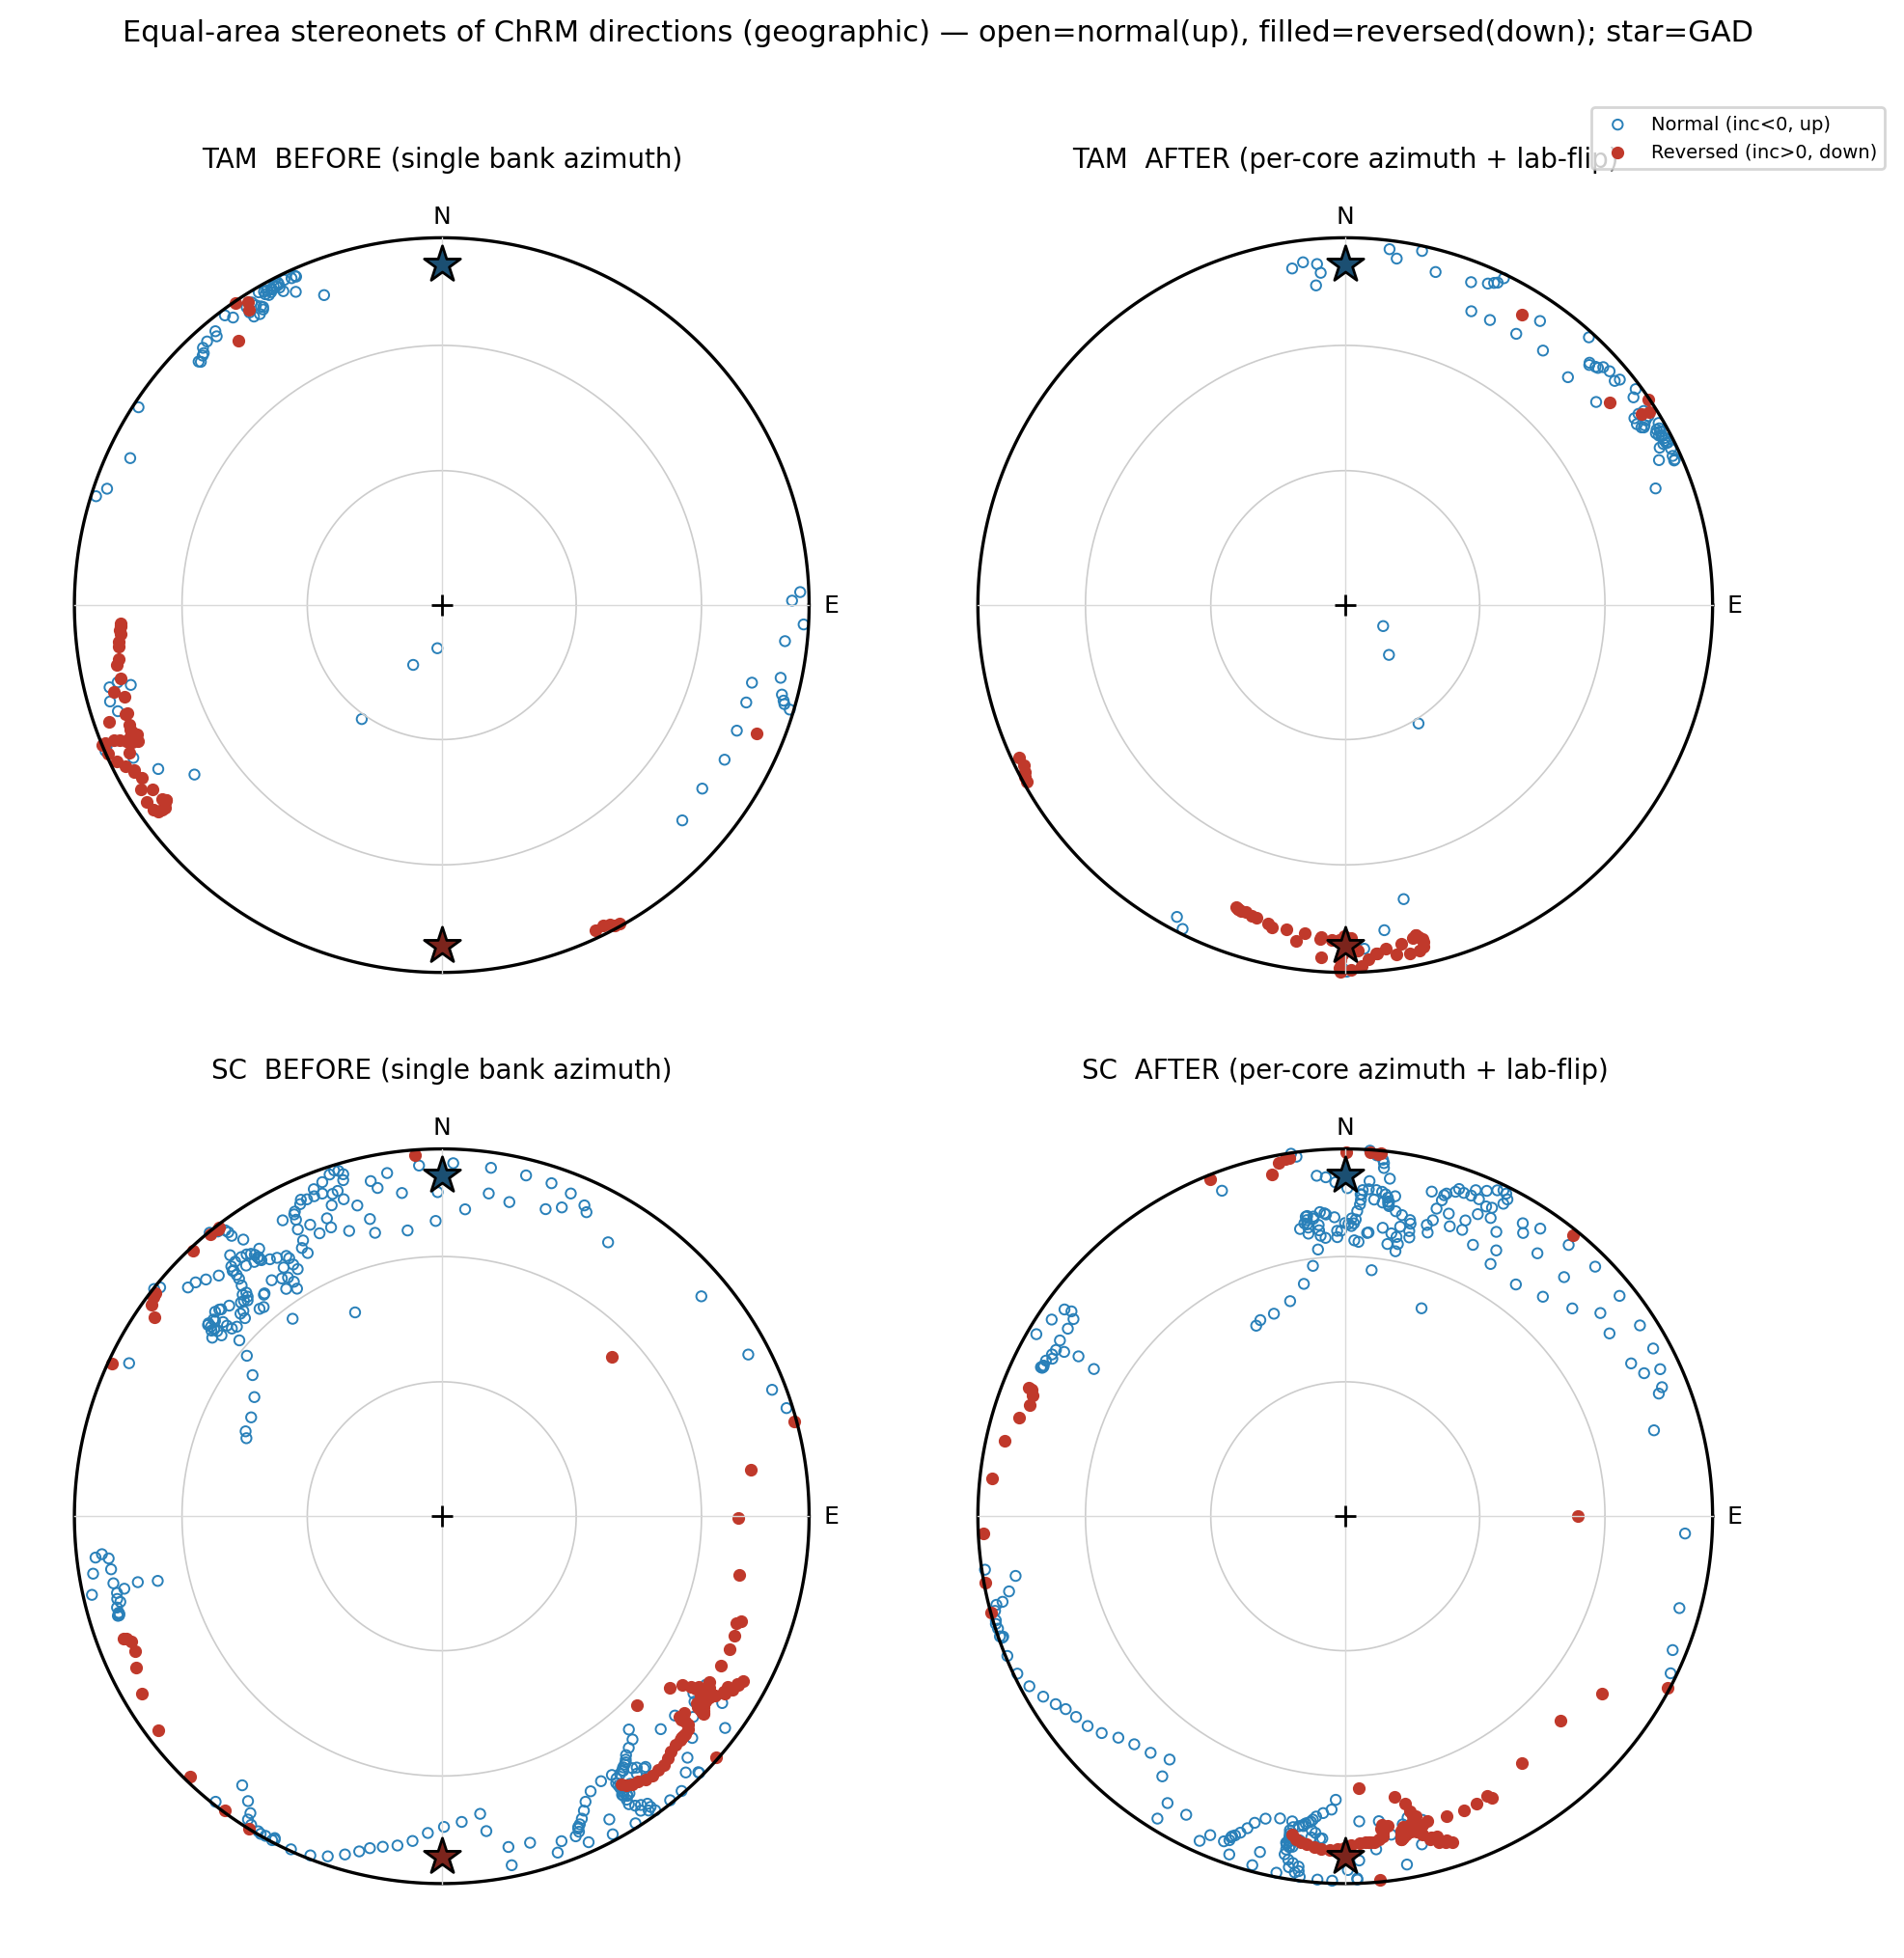
\includegraphics[width=\linewidth]{figs/fig_stereonet_dirs.png}
\caption{Equal-area stereonets of ChRM directions (geographic frame), before
(single bank azimuth) and after per-core azimuth reconstruction (with the binary
lab-flip resolved). Open $=$ normal (upward, $I<0$); filled $=$ reversed
(downward, $I>0$); stars $=$ expected GAD normal/reversed directions. After
reconstruction the directions collapse onto the N--S (declination $0/180^\circ$)
axis at the GAD directions.}
\label{fig:stereonet}
\end{figure}

\begin{figure}[htbp]\centering
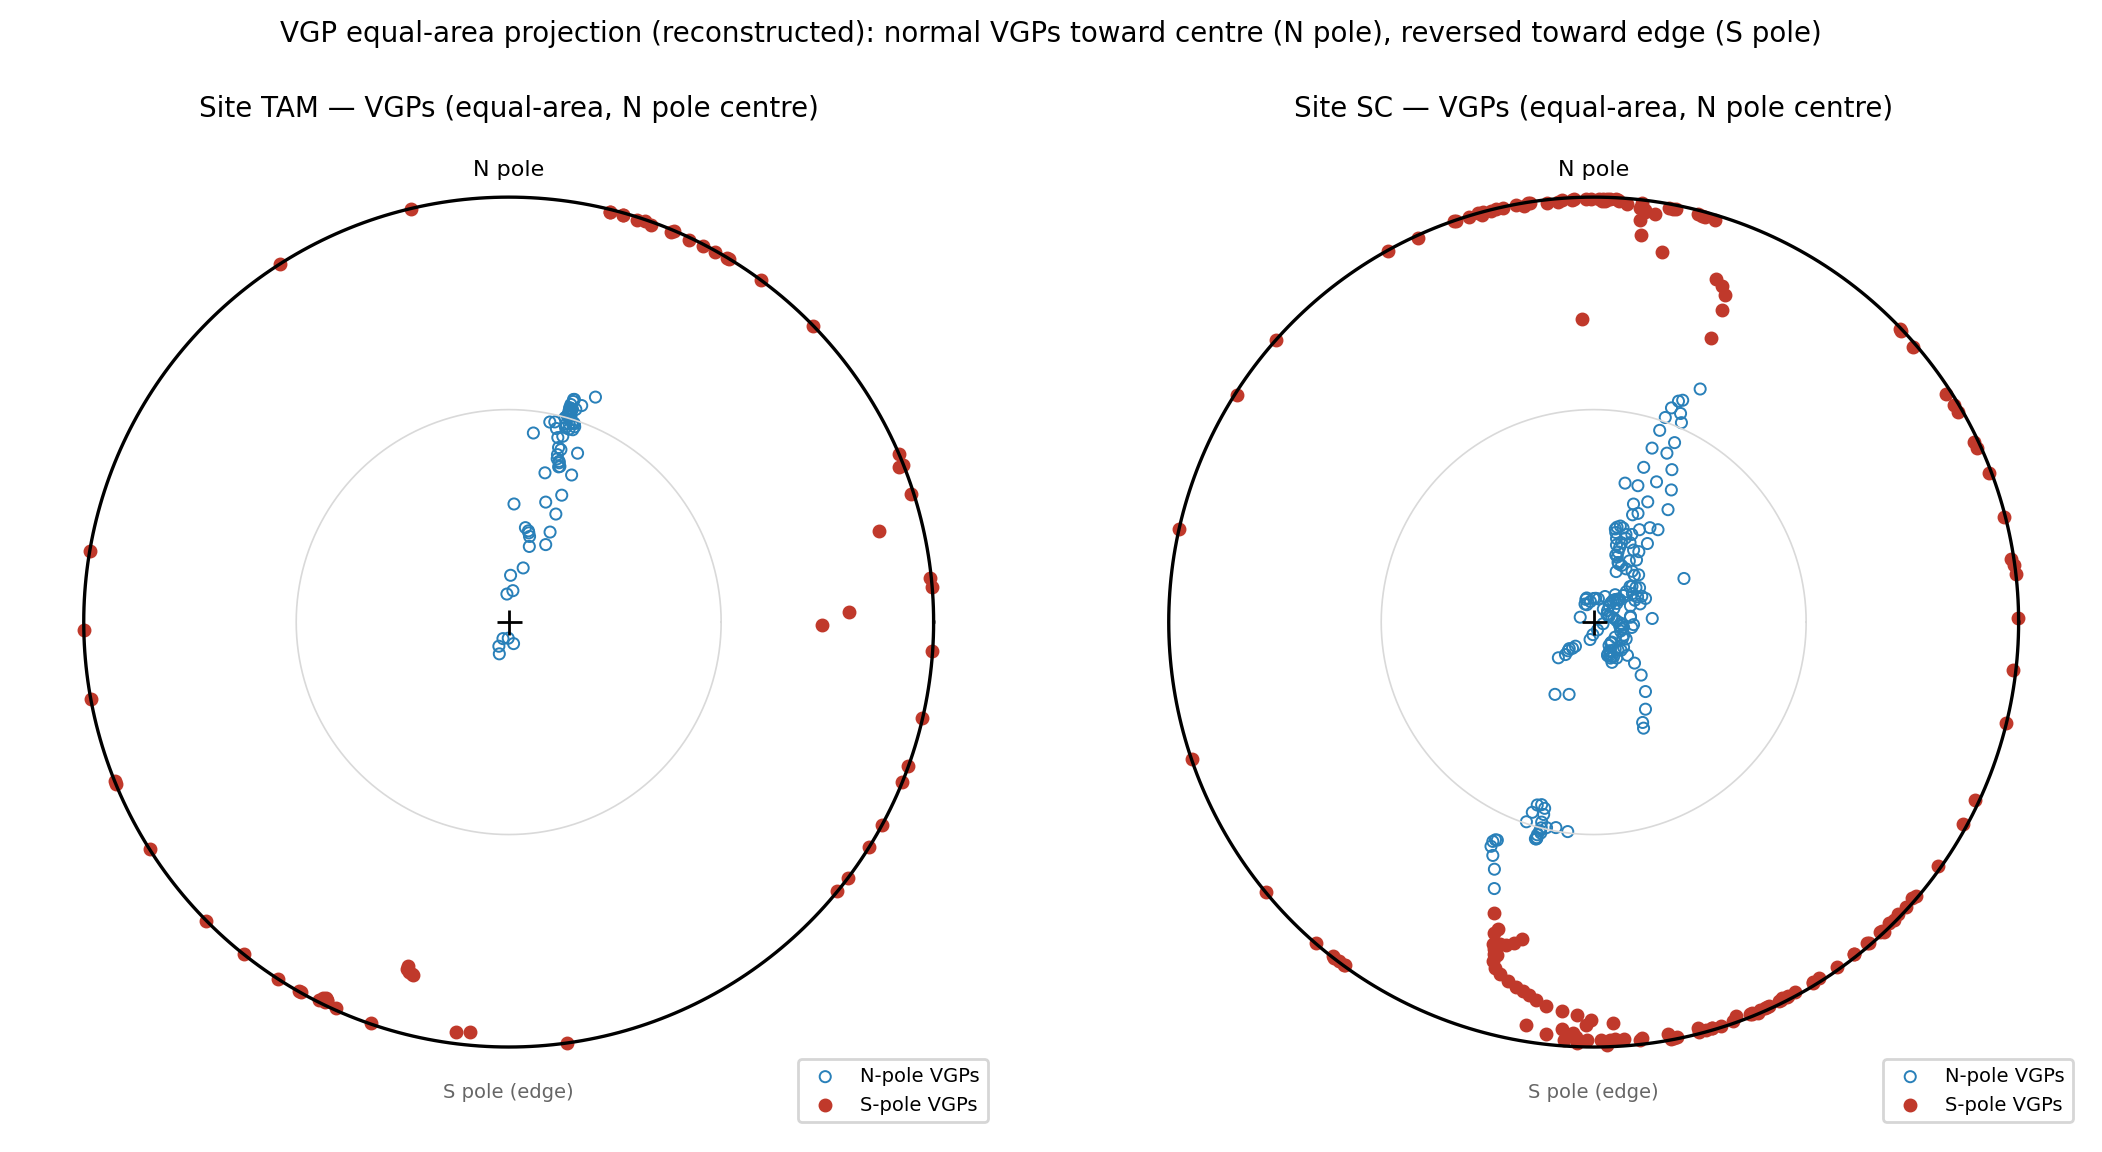
\includegraphics[width=\linewidth]{figs/fig_vgp_polar.png}
\caption{VGP equal-area projection (N pole at centre) of the reconstructed
directions. Normal-polarity VGPs (open) fall toward the centre (north pole) and
reversed VGPs (filled) toward the edge (south pole), for both sites.}
\label{fig:vgppolar}
\end{figure}

\subsection{Polarity records and internal correlation}
Foam-corrected composite polarity is:
\begin{itemize}
  \item \textbf{TAM}: (uppermost normal not preserved) $\to$ Reversed $\to$
        Normal ($\sim$\SI{99}{\centi\meter} of usable ChRM). The azimuth
        reconstruction additionally suggests the basal core TAM~7 is
        \emph{reversed} (Sec.~\ref{sec:vgp}); if confirmed with better
        demagnetization this would make the base of TAM Reversed--Normal--Reversed
        (a second, low reversal), but TAM~7 is currently low-quality and this
        remains tentative.
  \item \textbf{SC}: Normal $\to$ Reversed $\to$ Normal
        ($\sim$\SI{262}{\centi\meter}), with the reversal at
        \SIrange{106}{149}{\centi\meter} composite depth.
\end{itemize}
Each section records (at least) one well-resolved reversal, now confirmed in
both inclination and reconstructed declination; the most parsimonious
interpretation is that TAM's reversal (TAM-4) and SC's reversal (SC-4C$\to$4B)
are the same event. SC's Normal--Reversed--Normal thickness ratio
($103\!:\!43\!:\!88$\,cm) is best matched by a short reversed chron between two
long normals; a pattern-fit favours the C5AAr--C5ABr interval
($\sim$13.2--13.7\,Ma). TAM, having lost its uppermost
normal, is under-constrained on its own and is consistent with the same tie.

\begin{table}[h]\centering
\caption{Reversal reliability summary.}
\begin{tabular}{@{}llll@{}}
\toprule
Boundary & Inc.\ flip & Rel.\ decl.\ flip / antipodal & Verdict \\ \midrule
SC~4C$\to$4B & yes & yes ($\sim$\ang{157}) & \textbf{true reversal (high)} \\
TAM~3A$\to$4 & yes (gradual) & partial & true transition (moderate) \\
TAM~4$\to$5E & no & $\sim$\ang{182} & rotation artifact \\
TAM~5A$\to$6 & no & $\sim$\ang{140} & rotation artifact \\
TAM~6$\to$7 & possible & $\sim$\ang{188}$^{*}$ & possible N$\to$R reversal (tentative) \\
SC~7B & no & $\sim$\ang{180} & rotation artifact \\ \bottomrule
\end{tabular}

\medskip
{\footnotesize $^{*}$After azimuth reconstruction TAM~7 fits a reversed
direction for any orientation consistent with its neighbours, so the TAM~6/7
declination jump may be a genuine N$\to$R reversal rather than only a tray
rotation; TAM~7 is low-quality, so this is tentative.}
\end{table}

\begin{figure}[htbp]\centering
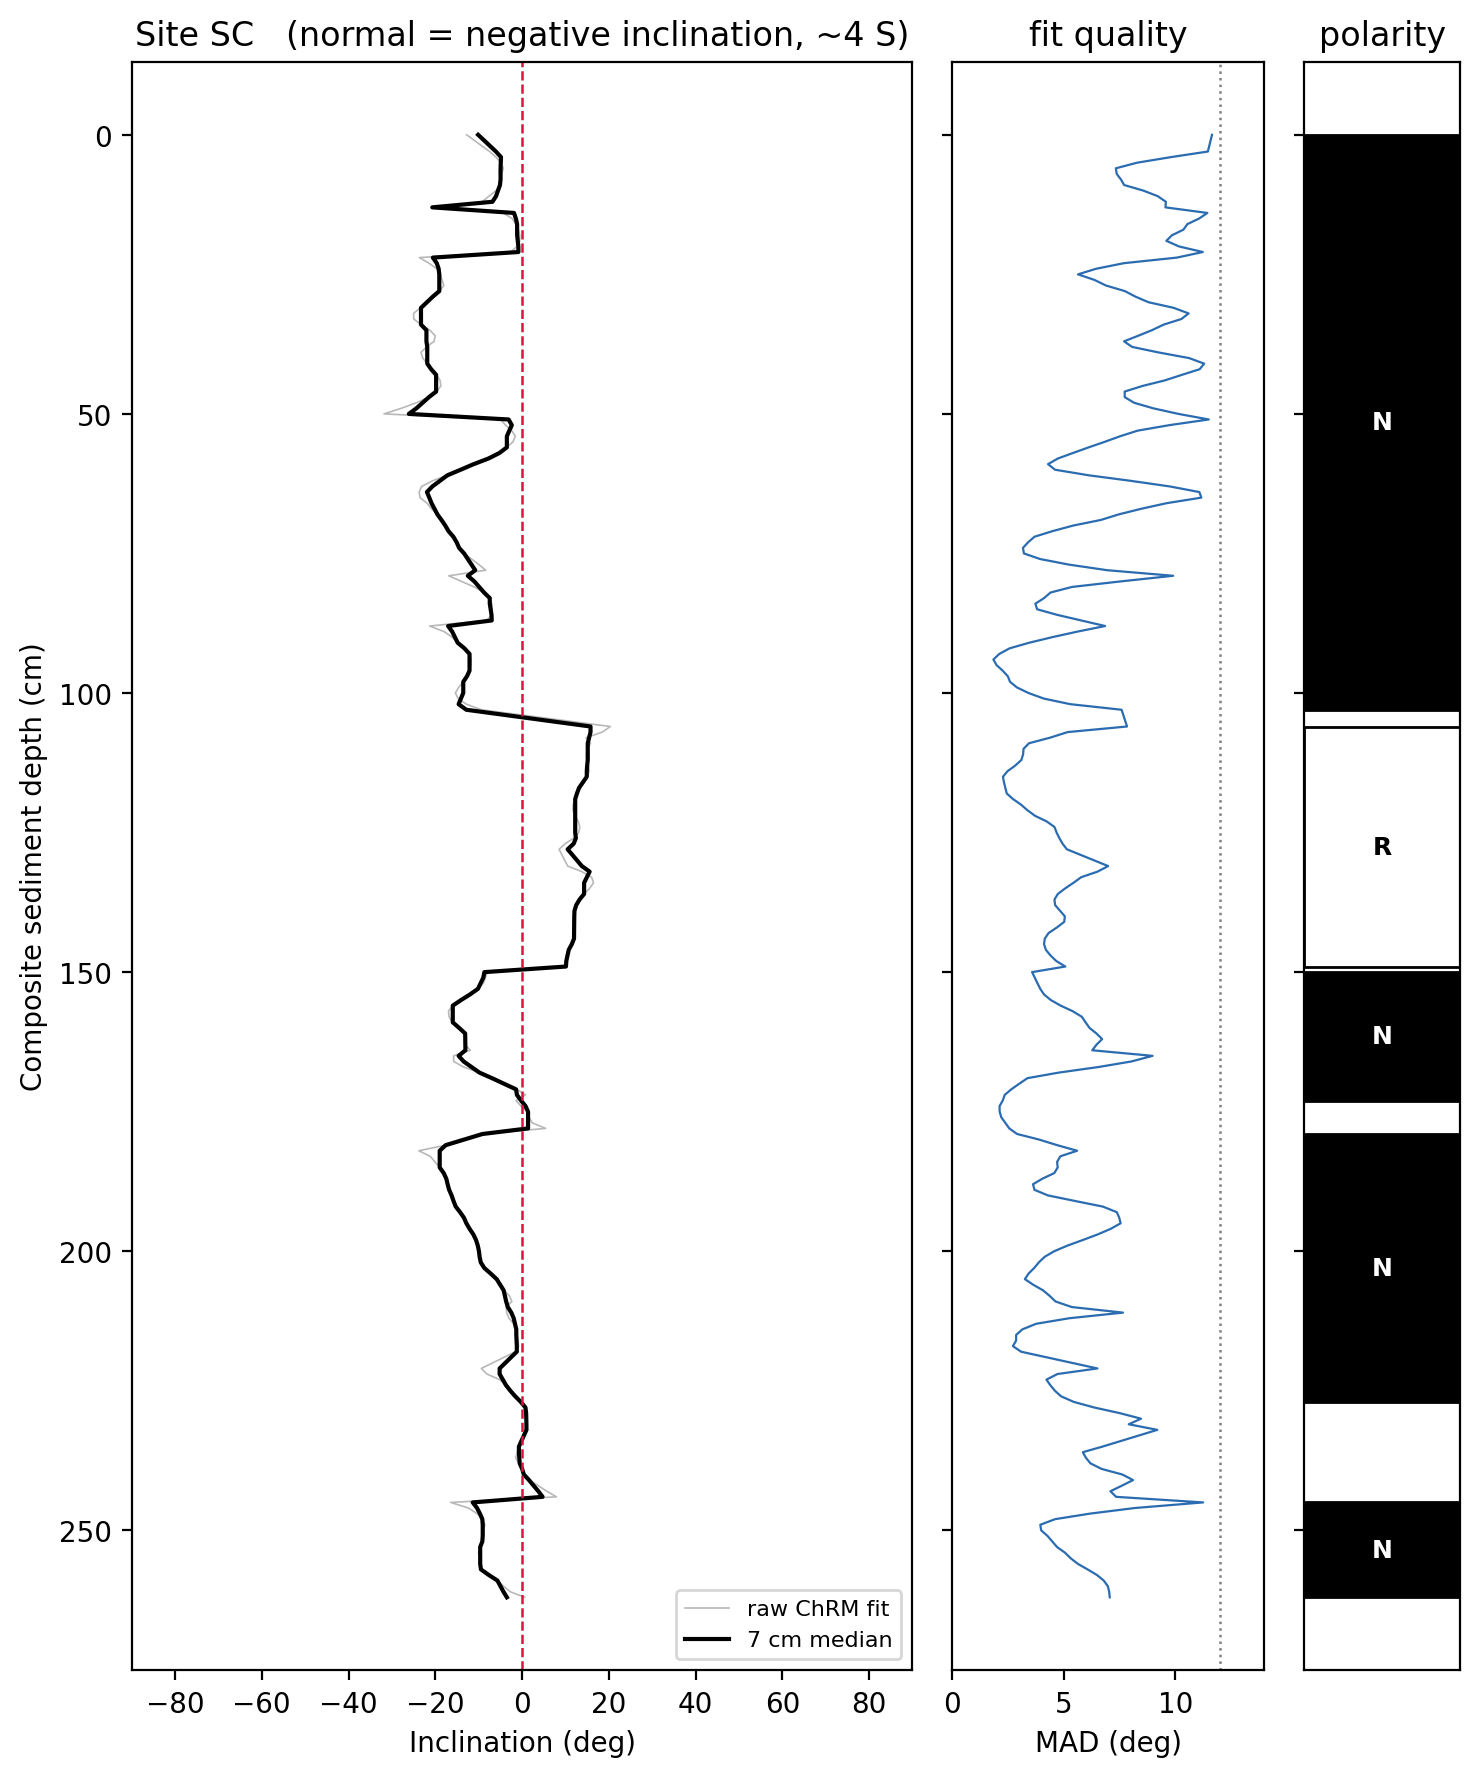
\includegraphics[width=0.49\linewidth]{figs/polarity_SC.png}\hfill
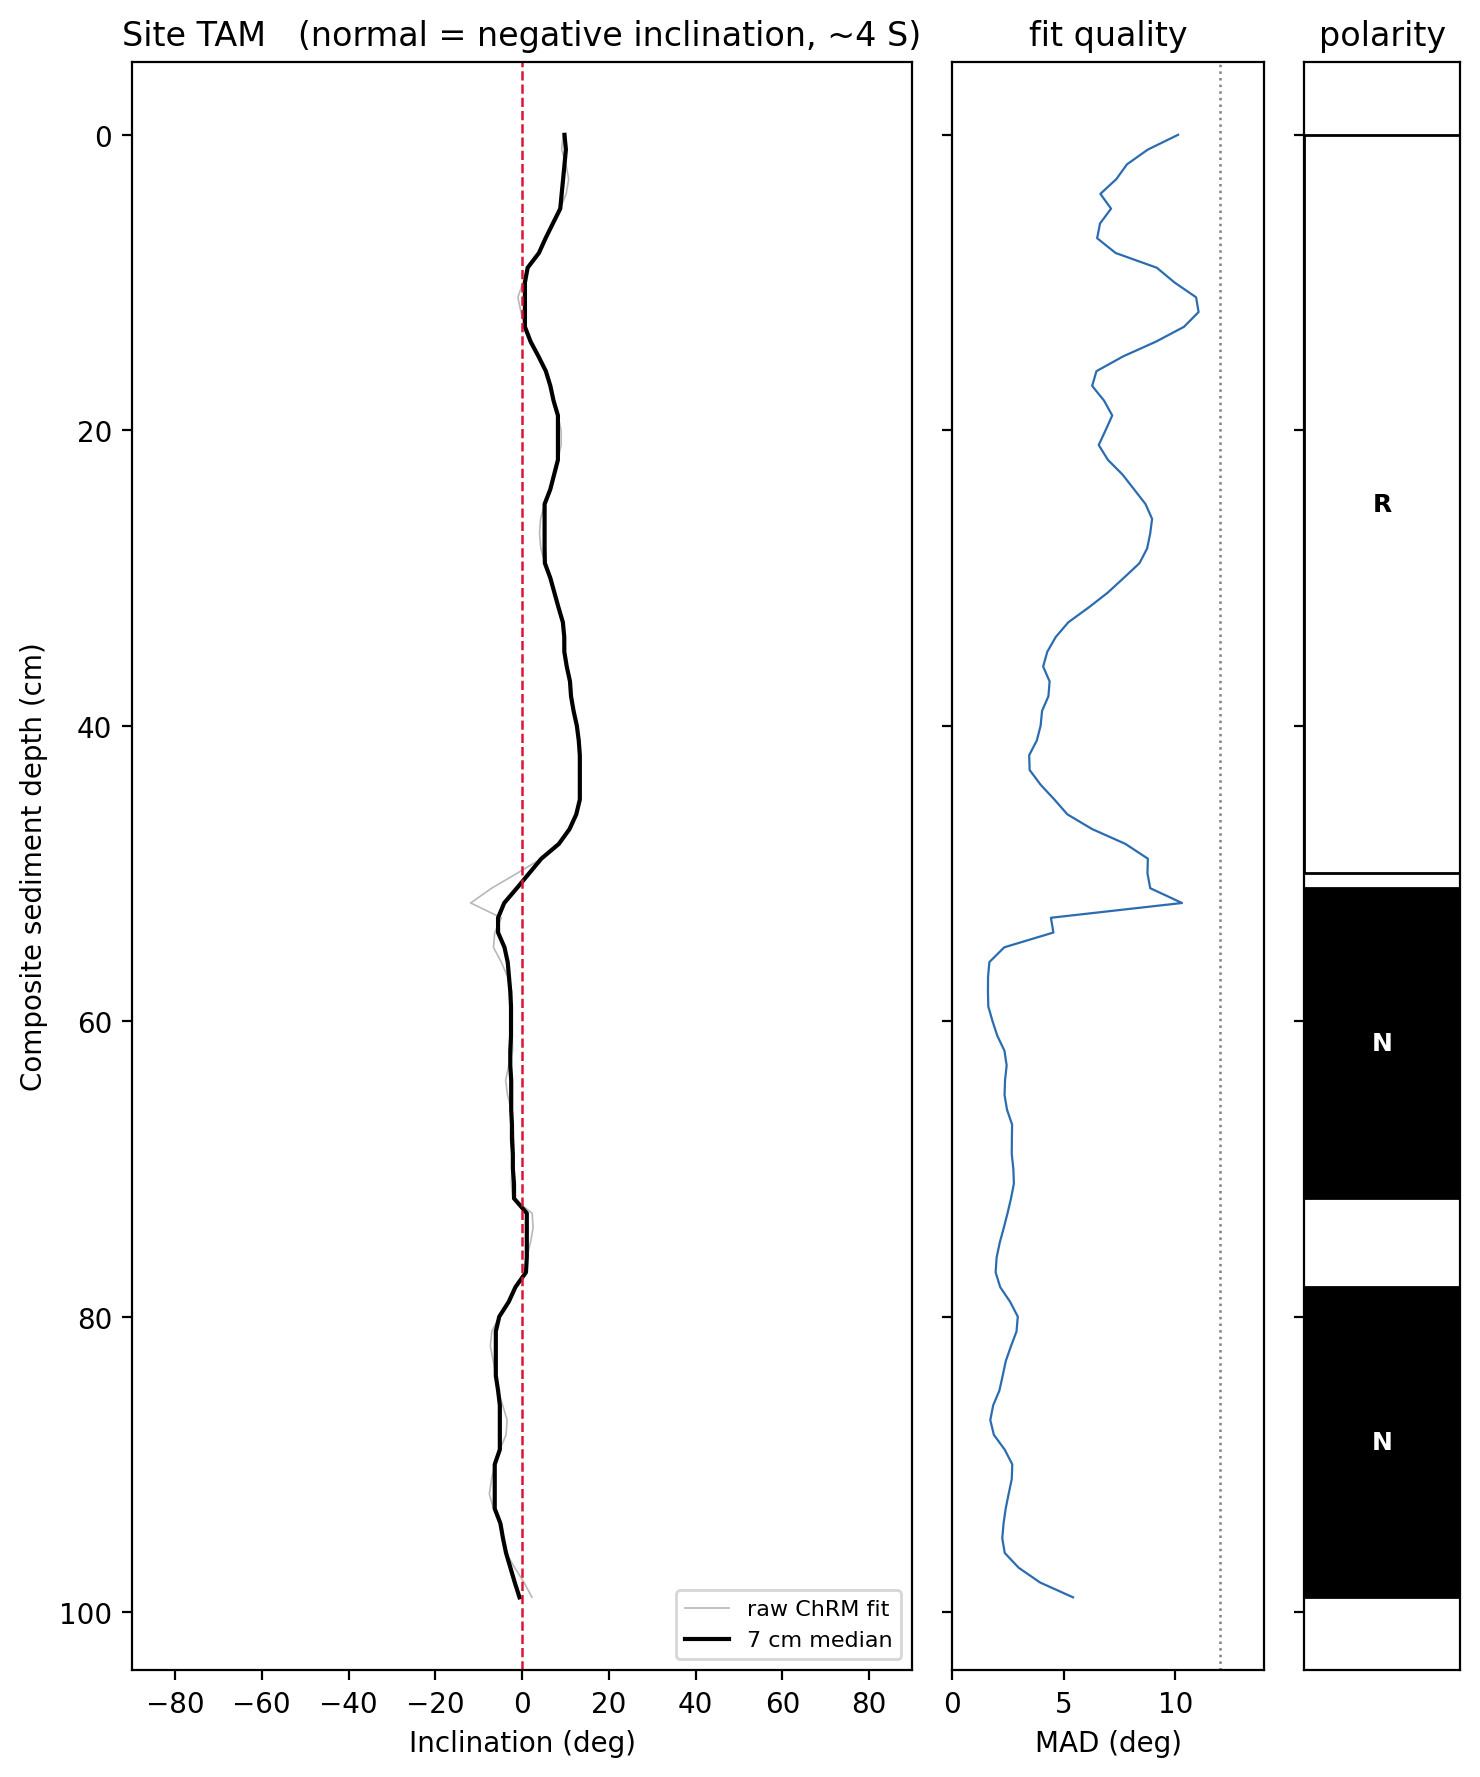
\includegraphics[width=0.49\linewidth]{figs/polarity_TAM.png}
\caption{Corrected ChRM inclination (raw grey; \SI{7}{\centi\meter} running
median black), MAD, and the resulting polarity column against composite
sediment depth for sites SC (left) and TAM (right). Normal polarity $=$
negative inclination at $\sim$\ang{4}\,S. SC records Normal--Reversed--Normal
with the reversal at \SIrange{106}{149}{\centi\meter}; TAM records
Reversed--Normal (its uppermost normal was not preserved; Group~1 excluded).}
\label{fig:polarity}
\end{figure}

\section{Rock-magnetic and XRF results}
NRM intensity co-varies with magnetic susceptibility in three of four matched
cores (log-intensity vs.\ susceptibility $r\approx0.5$--$0.75$; TAM~3A weaker at
$0.23$). Because susceptibility scales with magnetic-mineral concentration,
downcore intensity minima are interpreted as real sediment-property changes
(magnetite-poor, clay- or organic-rich intervals) rather than artifacts.
Two intervals show anomalously low or negative susceptibility --- SC~7C
(susceptibility $\sim$100$\times$ lower than adjacent cores) and SC~2
(diamagnetic) --- and carry correspondingly unreliable directions; these are
masked in the polarity interpretation.

The 27 XRF scans (1906 validity-filtered points) were depth-registered to the
paleomagnetic record per group (XRF position/10 $=$ measured u-channel
position). Contrary to the initial expectation that magnetic-mineral (Fe)
content would predict remanence intensity, \textbf{total Fe is only weakly and
inconsistently related to NRM intensity} (per-group Pearson $r$ on log-log
$-0.10$ to $+0.45$; pooled, within-group-standardized $r\approx+0.16$; Fe/Ti
$r\approx+0.08$). This is not a registration artifact: a depth-lag scan peaks
at zero offset and a coarse (\SI{5}{\centi\meter}-binned) comparison gives the
same weak result ($r\approx+0.18$).

Instead, \textbf{Fe co-varies with S and Ca}: log Fe vs.\ log S reaches
$r=+0.5$--$0.7$ (pooled $+0.39$) and log Fe vs.\ log Ca reaches $r=+0.7$--$0.9$
(pooled $+0.56$). We interpret this to mean that in this organic-rich,
reducing, lignitic facies most iron resides in \emph{authigenic} phases ---
pyrite (Fe--S) and carbonate/shell-associated or Fe-carbonate intervals
(Fe--Ca) --- rather than in detrital magnetite. Total Fe measured by XRF is
therefore a poor proxy for the remanence carrier here, which is why it fails to
track NRM intensity even though \emph{susceptibility} does
($r\approx0.5$--$0.75$; above). The two groups with the strongest Fe--intensity
coupling (TAM~5B--5A--6--7, $r\approx0.45$; SC~3B--3A--4, $r\approx0.27$) are
also those with the strongest Fe--S/Fe--Ca signal, i.e.\ where a larger
detrital component is preserved.

The implication is that reductive diagenesis (pyritisation) exerted a
first-order control on the magnetic mineralogy: it both sequestered iron into
pyrite and diluted or dissolved the detrital magnetite that carries the
remanence, producing the low-intensity, low-susceptibility intervals. The
lithological control on remanence intensity is thus real, but it is diagnosed
by susceptibility, not by XRF Fe; XRF instead resolves the diagenetic
(pyrite) and carbonate/detrital architecture of the section. Downcore profiles
and cross-plots are given below (Figs~\ref{fig:xrf_pyrite},
\ref{fig:xrf_downhole}).

\begin{figure}[htbp]\centering
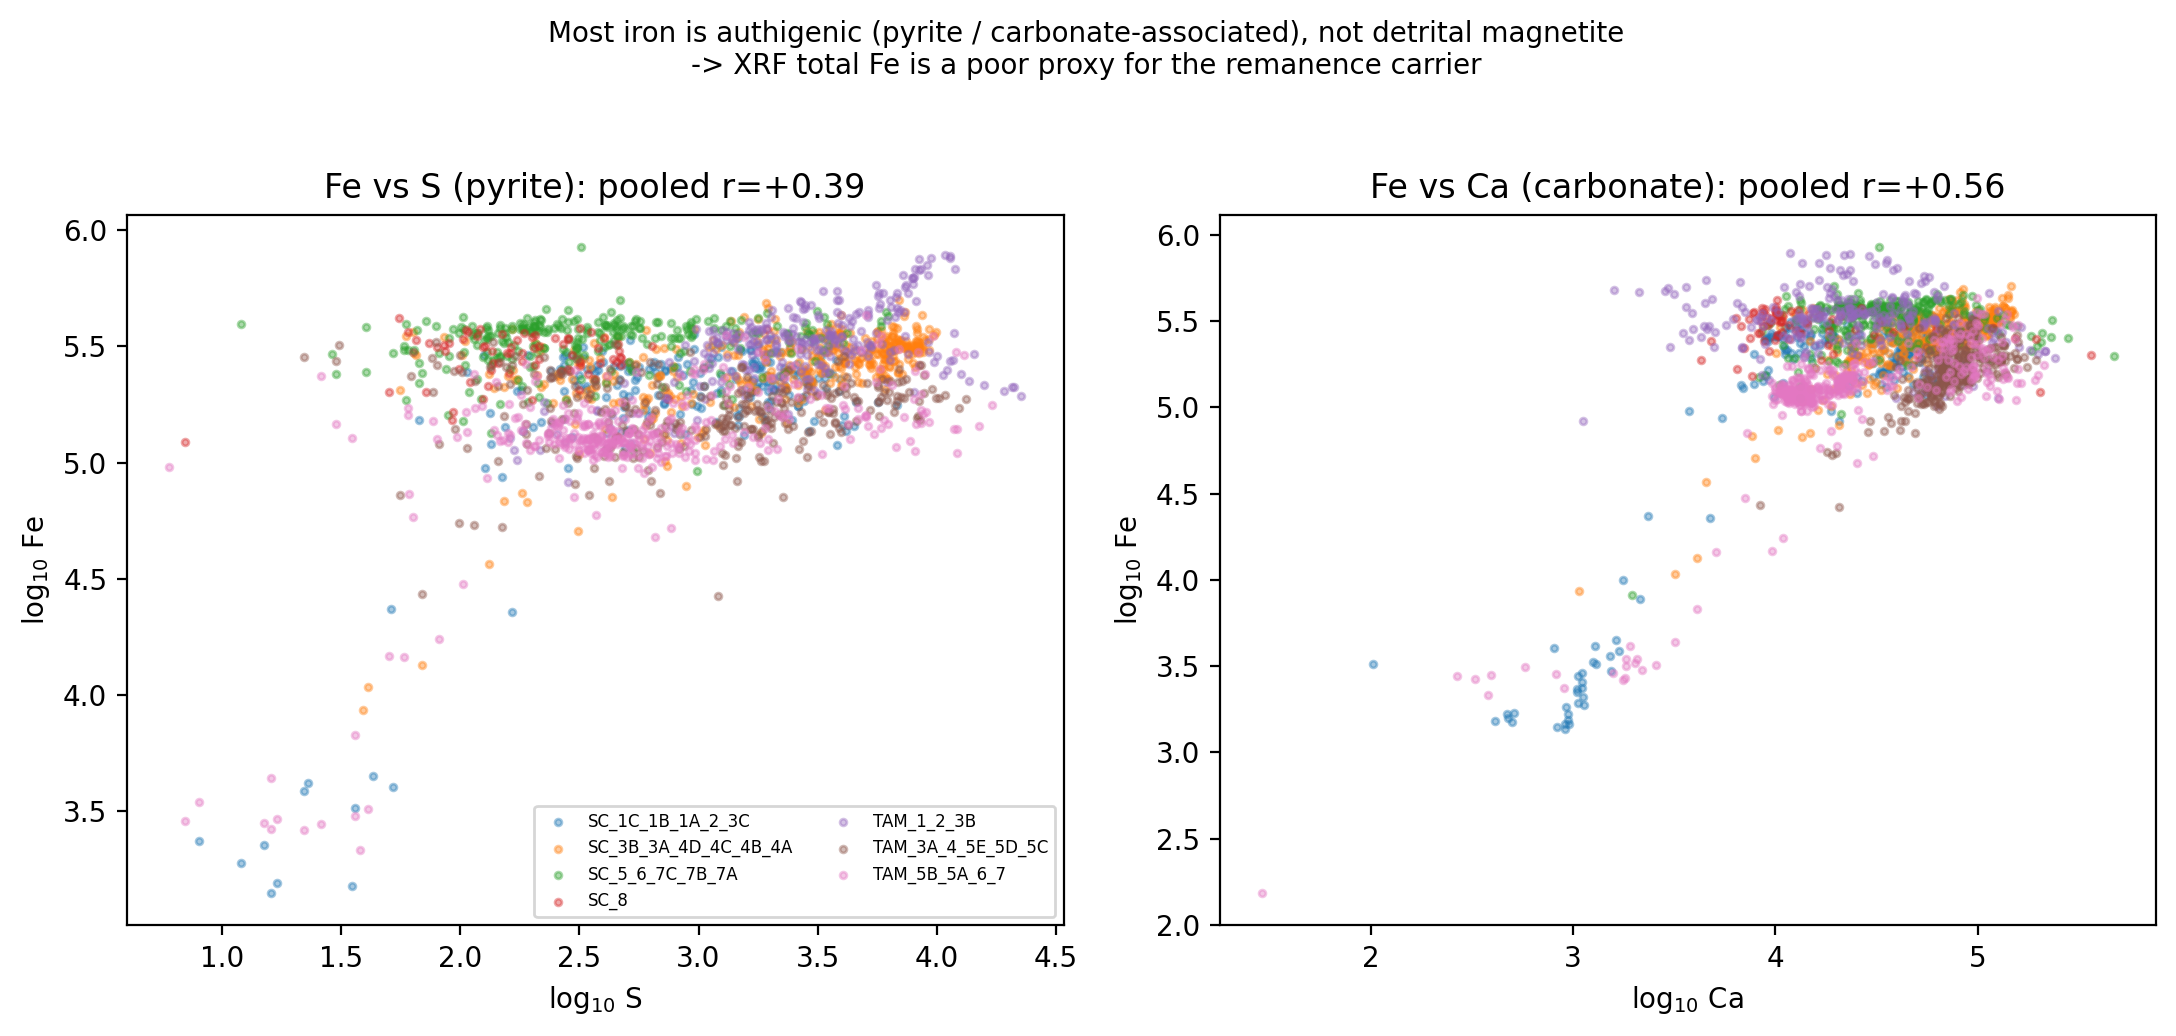
\includegraphics[width=\linewidth]{figs/fig_xrf_pyrite.png}
\caption{XRF total Fe co-varies with S (pyrite; pooled $r=+0.39$) and Ca
(carbonate; pooled $r=+0.56$), indicating that most iron is authigenic rather
than detrital magnetite. This is why total Fe does not predict the
magnetite-controlled remanence intensity.}
\label{fig:xrf_pyrite}
\end{figure}

\begin{figure}[htbp]\centering
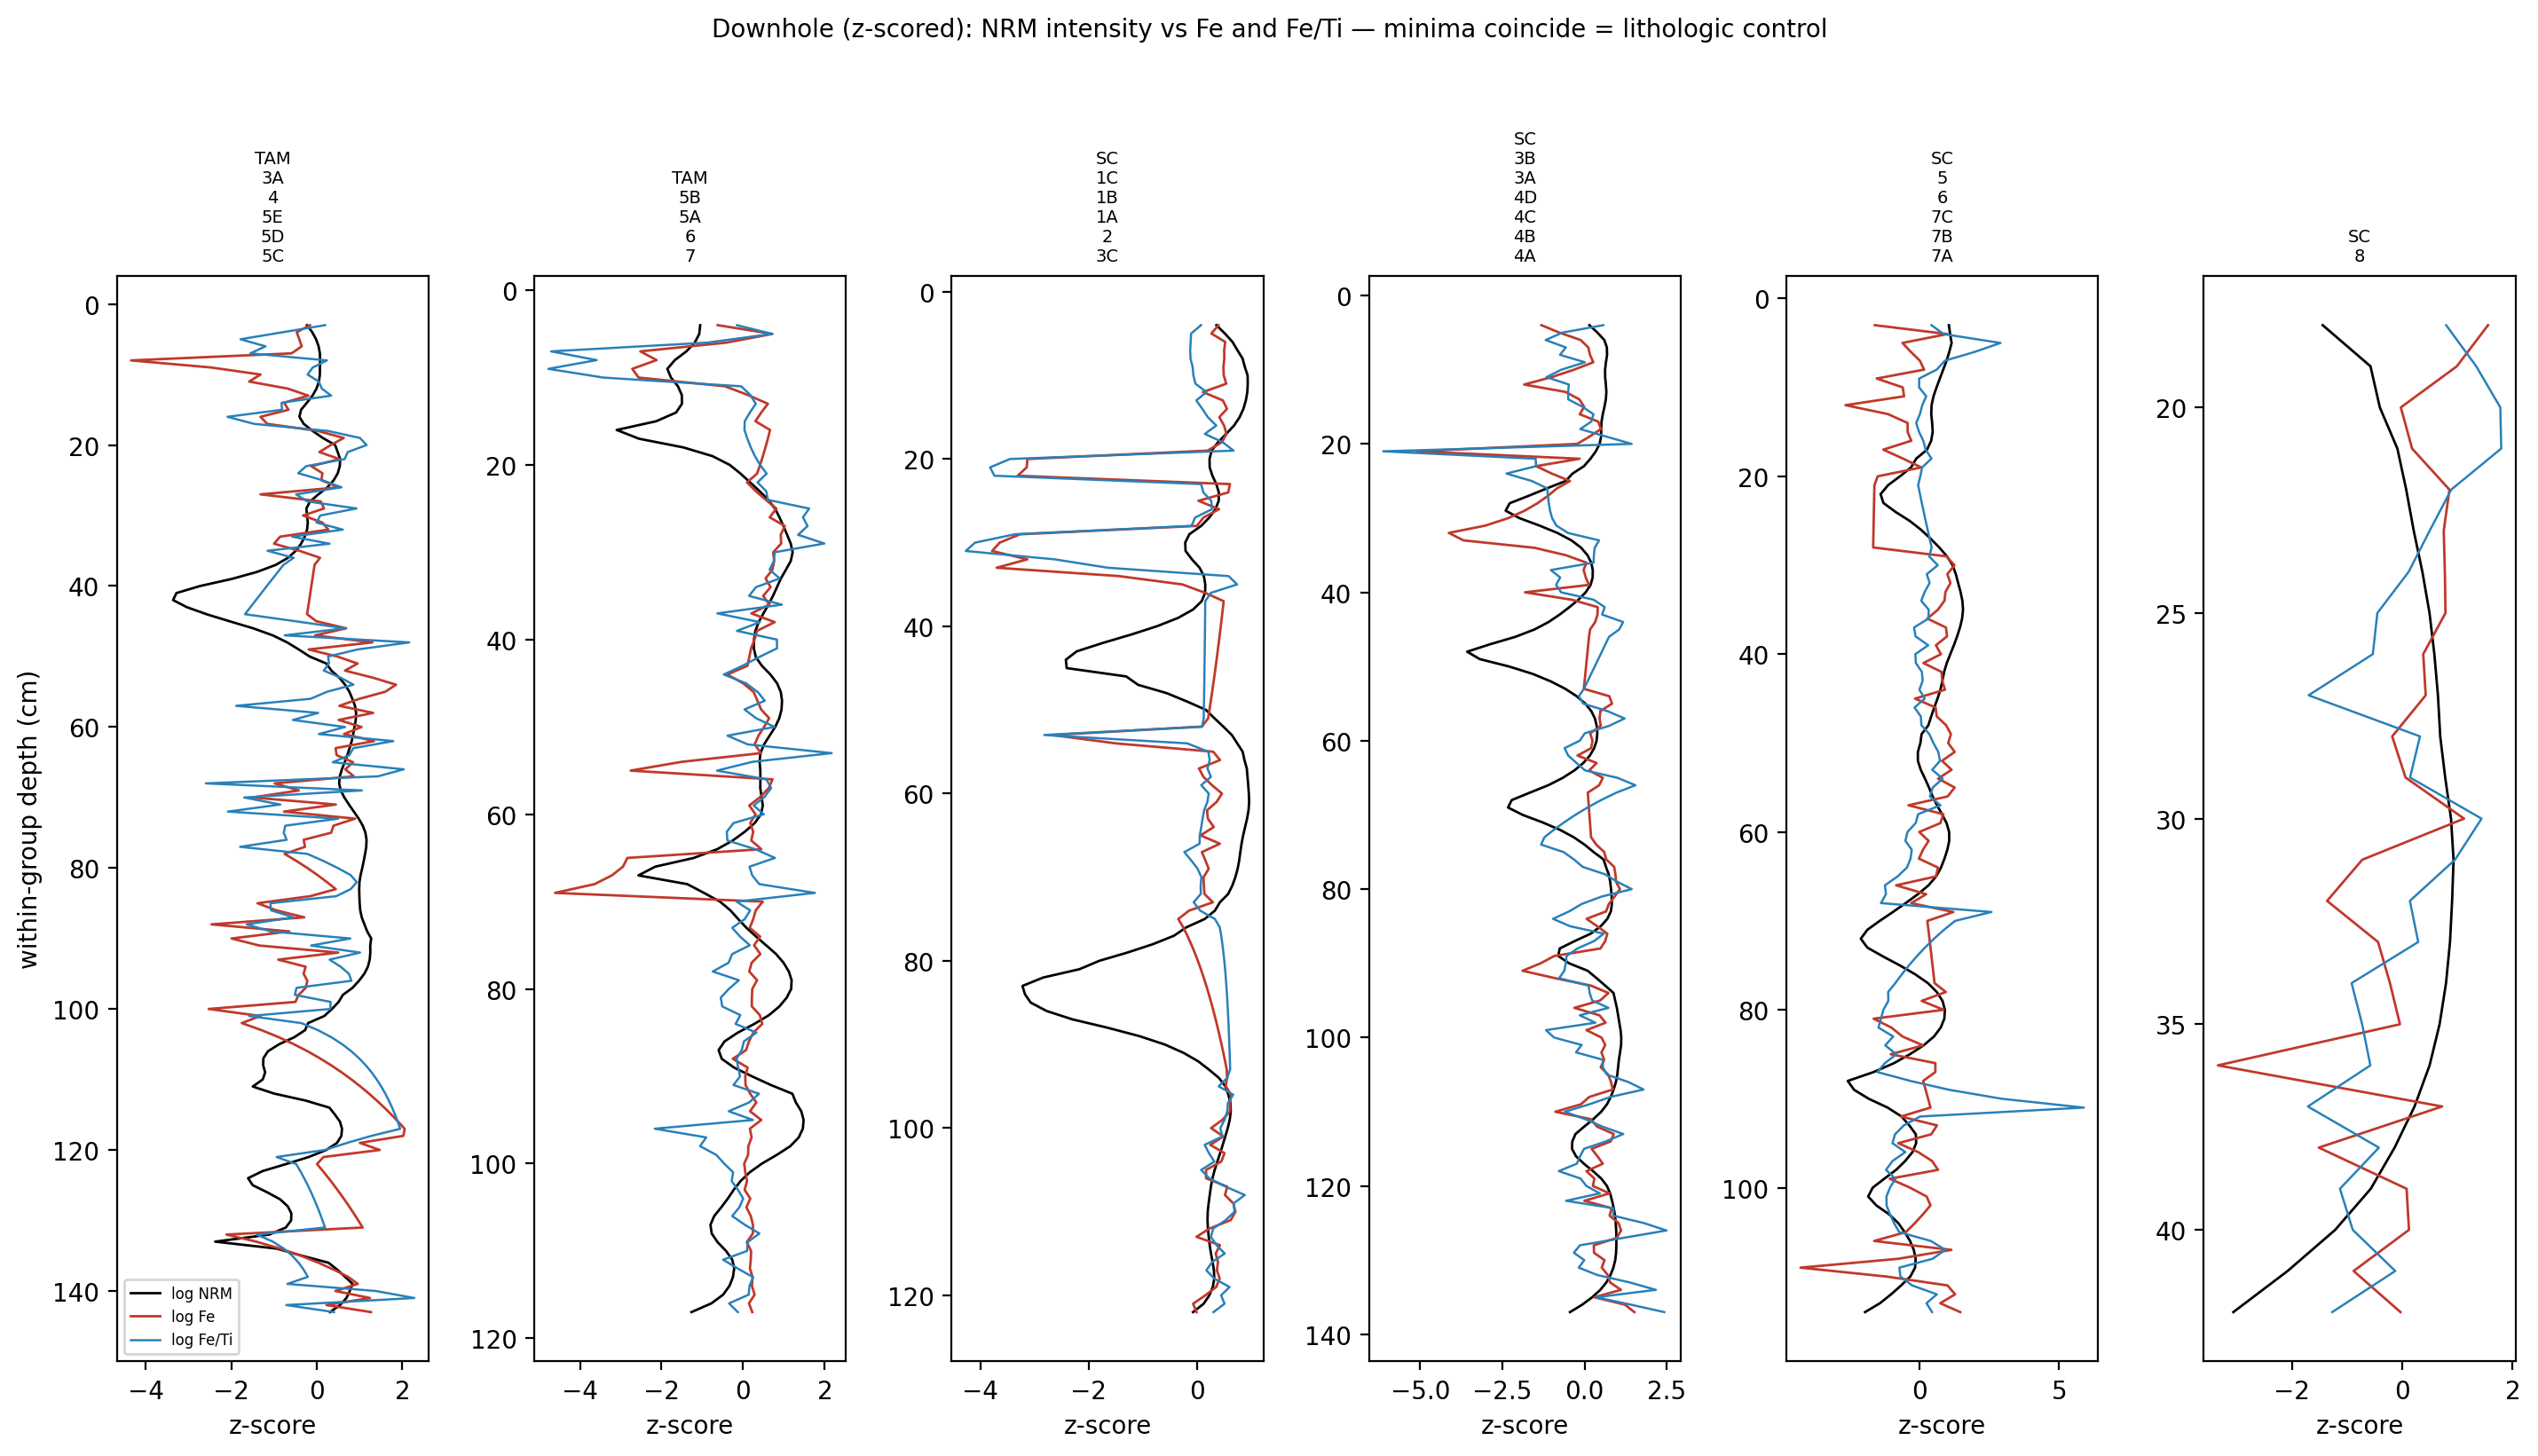
\includegraphics[width=\linewidth]{figs/fig_xrf_downhole.png}
\caption{Downhole (within-group $z$-scored) NRM intensity vs.\ Fe and Fe/Ti.
The lack of consistent coincidence between intensity and Fe minima confirms
that XRF Fe is a poor proxy for the remanence carrier; susceptibility (not
shown) remains the reliable magnetic-concentration proxy.}
\label{fig:xrf_downhole}
\end{figure}

\subsection{Elemental stratigraphy}\label{sec:elemstrat}
Downcore, the elements most diagnostic of the depositional environment vary by
one to two orders of magnitude and co-vary systematically (Fig.~\ref{fig:paleoenv}).
Sulphur (pyrite) ranges over $\sim$two orders of magnitude (10th--90th percentile
$\sim$110--\SI{6000}{} peak-area units) and is highest in discrete, decimetre-scale
intervals; Fe and Ca track those same intervals (pooled log--log $r$: Fe--S
$=+0.39$, Fe--Ca $=+0.56$, S--Ca $=+0.57$), and Ca in turn co-varies with Sr
($r=+0.62$), the expected signature of aragonitic mollusc carbonate. Fe/Ti
(authigenic-Fe enrichment above the detrital baseline) rises in the same
pyrite-and-carbonate-rich intervals, whereas K/Ti (a clay/detrital proxy) is
comparatively flat, indicating the elemental variability is driven by authigenic
mineral formation rather than changing detrital provenance. Manganese, mobile
under reducing pore-waters, is low in the most pyritic intervals.

\begin{figure}[htbp]\centering
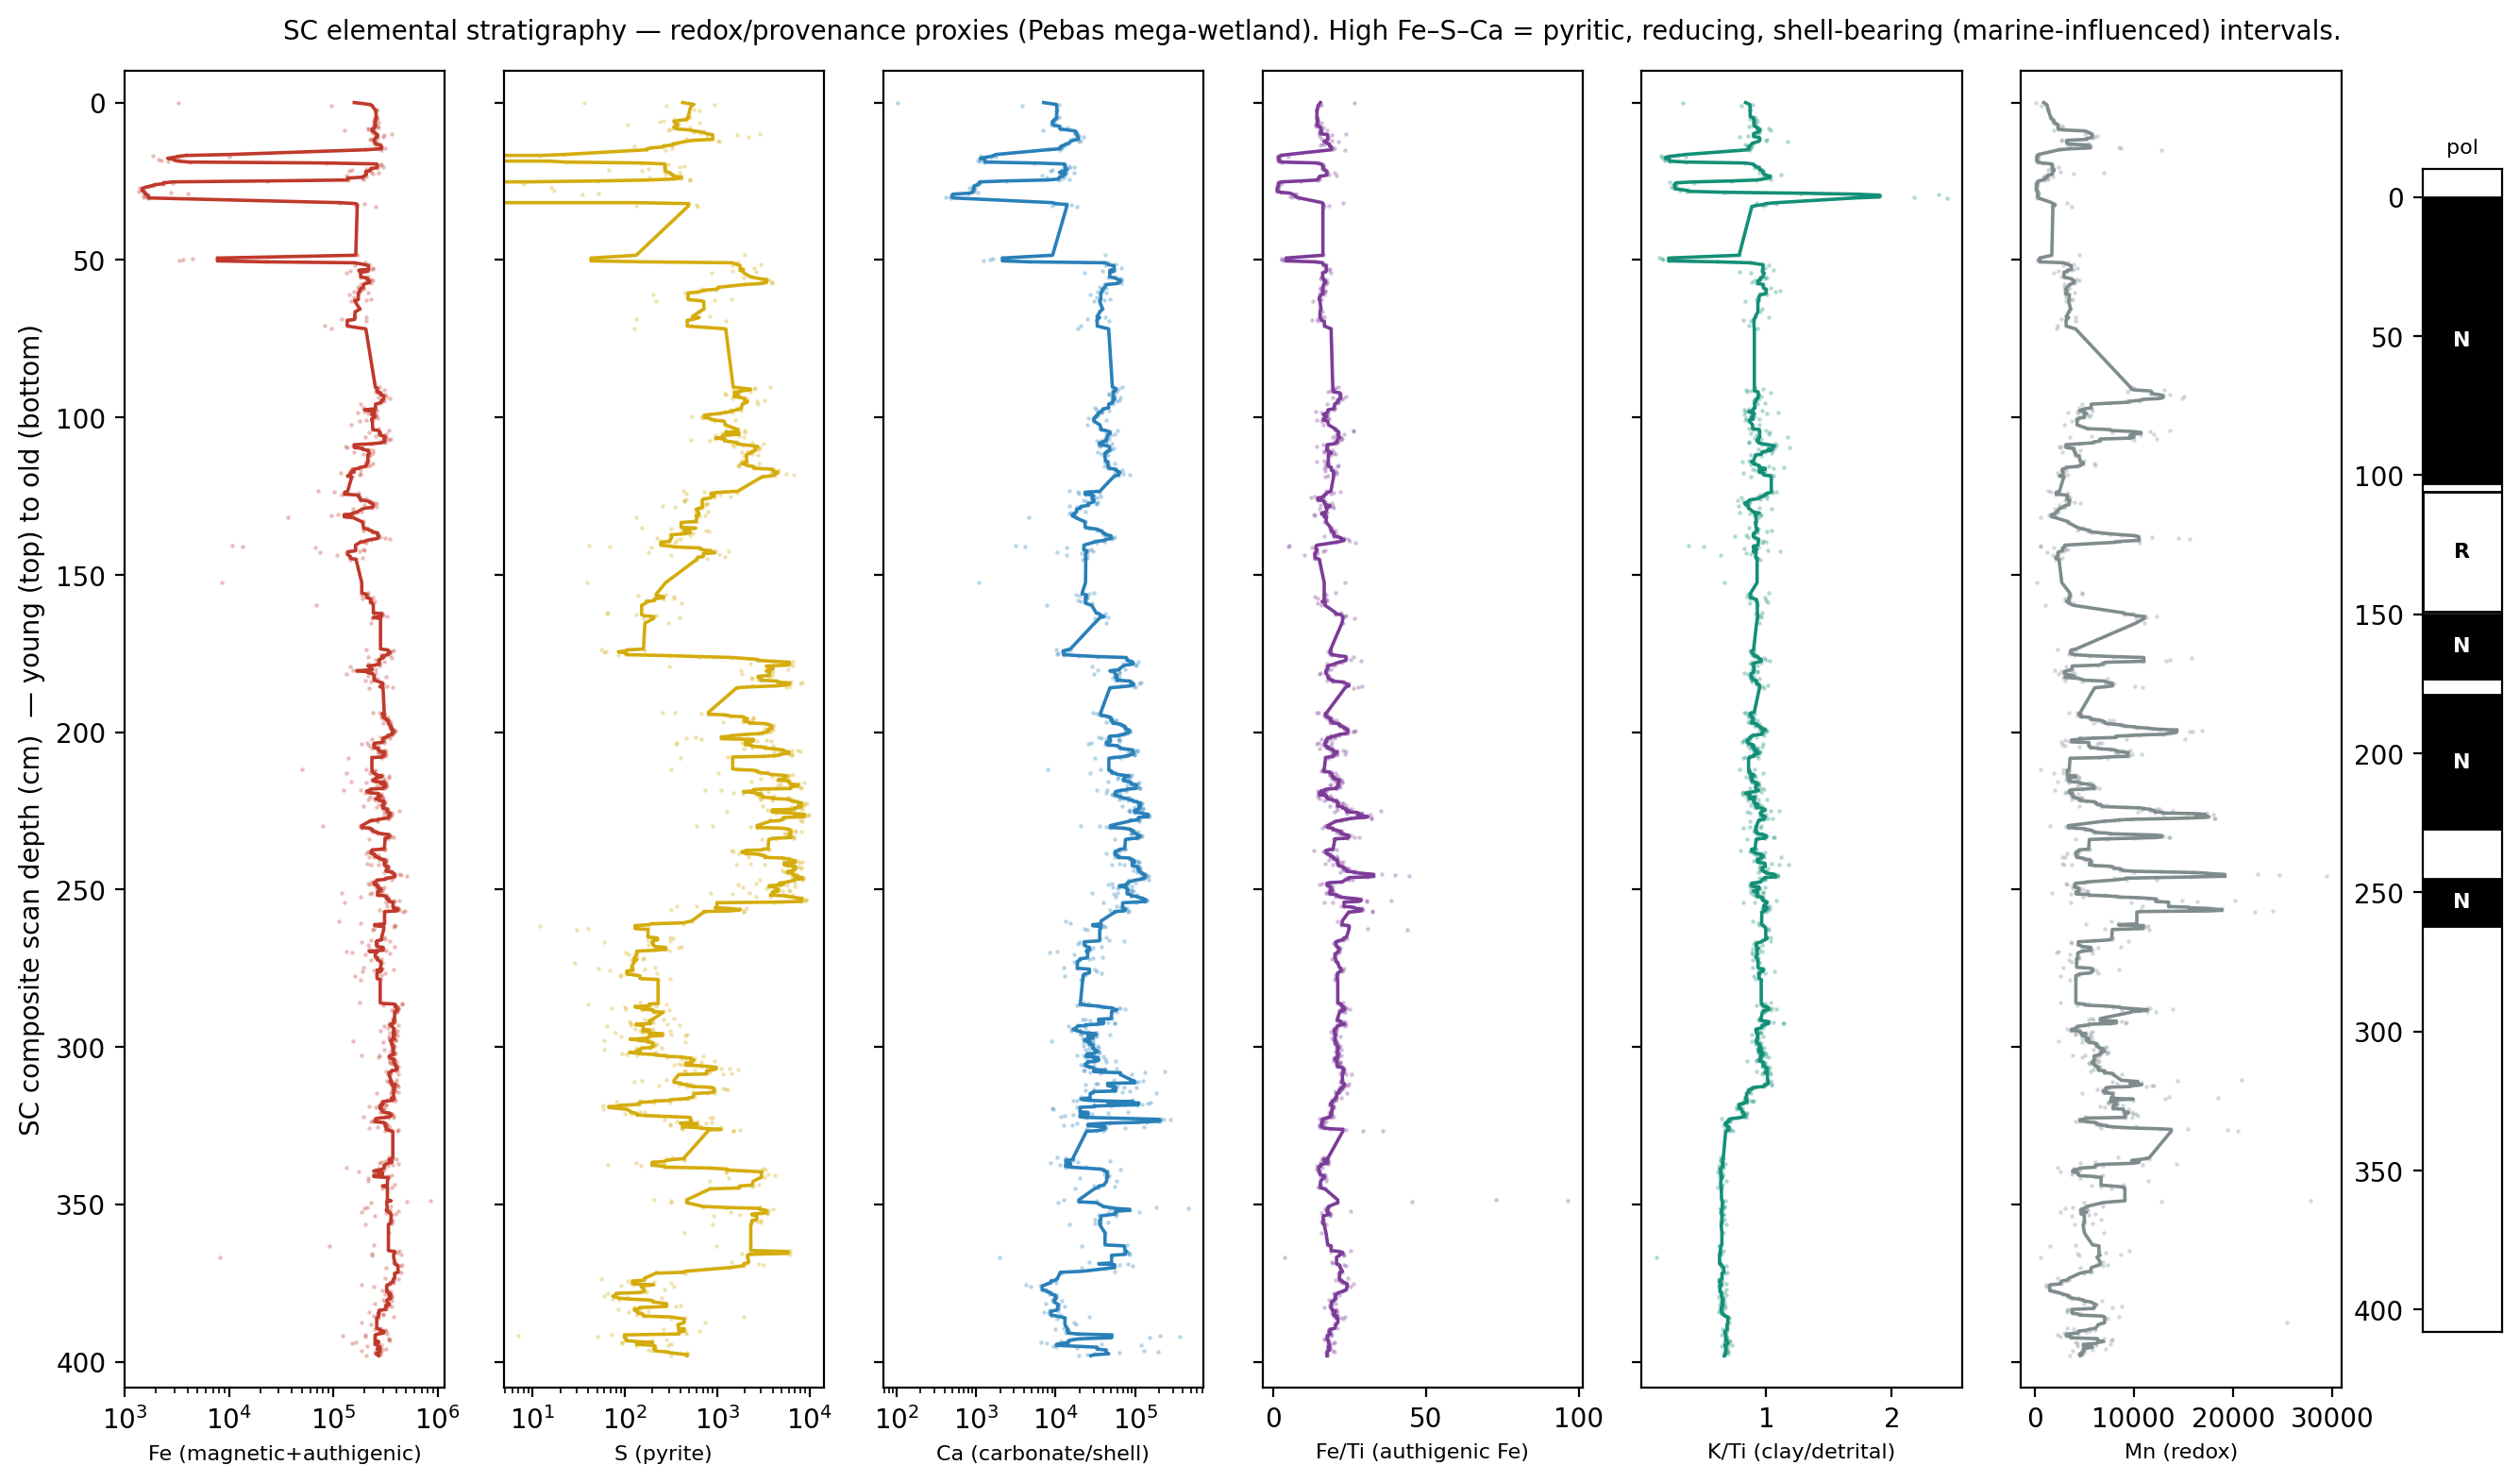
\includegraphics[width=\linewidth]{figs/fig_xrf_paleoenv.png}
\caption{Elemental stratigraphy of the SC composite (valid XRF points; running
median). Sulphur (pyrite), Fe and Ca (carbonate/shell, with Sr) are enriched
together in discrete reducing intervals; Fe/Ti (authigenic Fe) tracks them while
K/Ti (detrital) stays flat and Mn (redox) is depressed. Polarity column at right.
Depth is approximate composite scan depth (young at top).}
\label{fig:paleoenv}
\end{figure}

\section{Fossil age control: \textit{Purussaurus}}\label{sec:fossil}
A fossil of the giant caiman \textit{Purussaurus} was recovered at TAM
approximately \SI{0.5}{\meter} above the base of the measured section.
\textit{Purussaurus} is a middle-to-late Miocene genus whose oldest records
($\sim$13\,Ma; \textit{P.\ neivensis}) occur at La Venta
(Colombia) and in the Pebas Formation near Iquitos, where \textit{P.\
neivensis} is the apex predator of a $\sim$13\,Ma crocodylian
assemblage dated by palynology and mollusc/ostracod zonation
\citep{SalasGismondi2015,Pujos2020}. The genus therefore imposes a maximum-age
(older) bound of $\sim$13.8\,Ma on the fossil horizon --- the
complement of the palynological T-15/T-16 minimum-age bound of
12.7\,Ma. Together these independent constraints bracket the
section to $\sim$12.7--13.8\,Ma (and, using the
$\sim$13\,Ma Iquitos-Pebas assemblage age, to
$\sim$12.7--13.0\,Ma), consistent with the magnetostratigraphic
correlation to C5AAr--C5ABr (Fig.~\ref{fig:puru}). The independent, U-Pb-based
refinement of this ceiling from La Venta is developed in
Section~\ref{sec:laventa}.

Caveats: (i) genus-level identification alone permits only the broad mid--late
Miocene ($\sim$13--6.8\,Ma) range; the tight bound requires
species identification, as only \textit{P.\ neivensis} is diagnostically
middle Miocene (a late Miocene species --- \textit{P.\ mirandai},
\textit{P.\ brasiliensis} --- would falsify the $\sim$13\,Ma
reading). (ii) Because \textit{Purussaurus} in Amazonia is partly calibrated by
the Pebas itself, the independent leg of the argument is La Venta, where
\textit{P.\ neivensis} is now dated by U-Pb zircon geochronology
(Section~\ref{sec:laventa}; \citealp{MoraRojas2023}), not only mammal
biostratigraphy. (iii) The fossil
lies in the (excluded) Group~1 interval, so it presently anchors the section as
a whole rather than a specific polarity zone.

The Pebas facies (blue-grey lignitic clays, Pebasian fauna) together with this
Pebas-fauna vertebrate exclude a younger fluvial-terrace or Nauta-Formation
origin for the section; the terrace, Nauta, and Madre-de-Di\'os units of the
region overlie, and are younger than, the sediments studied here.

\begin{figure}[htbp]\centering
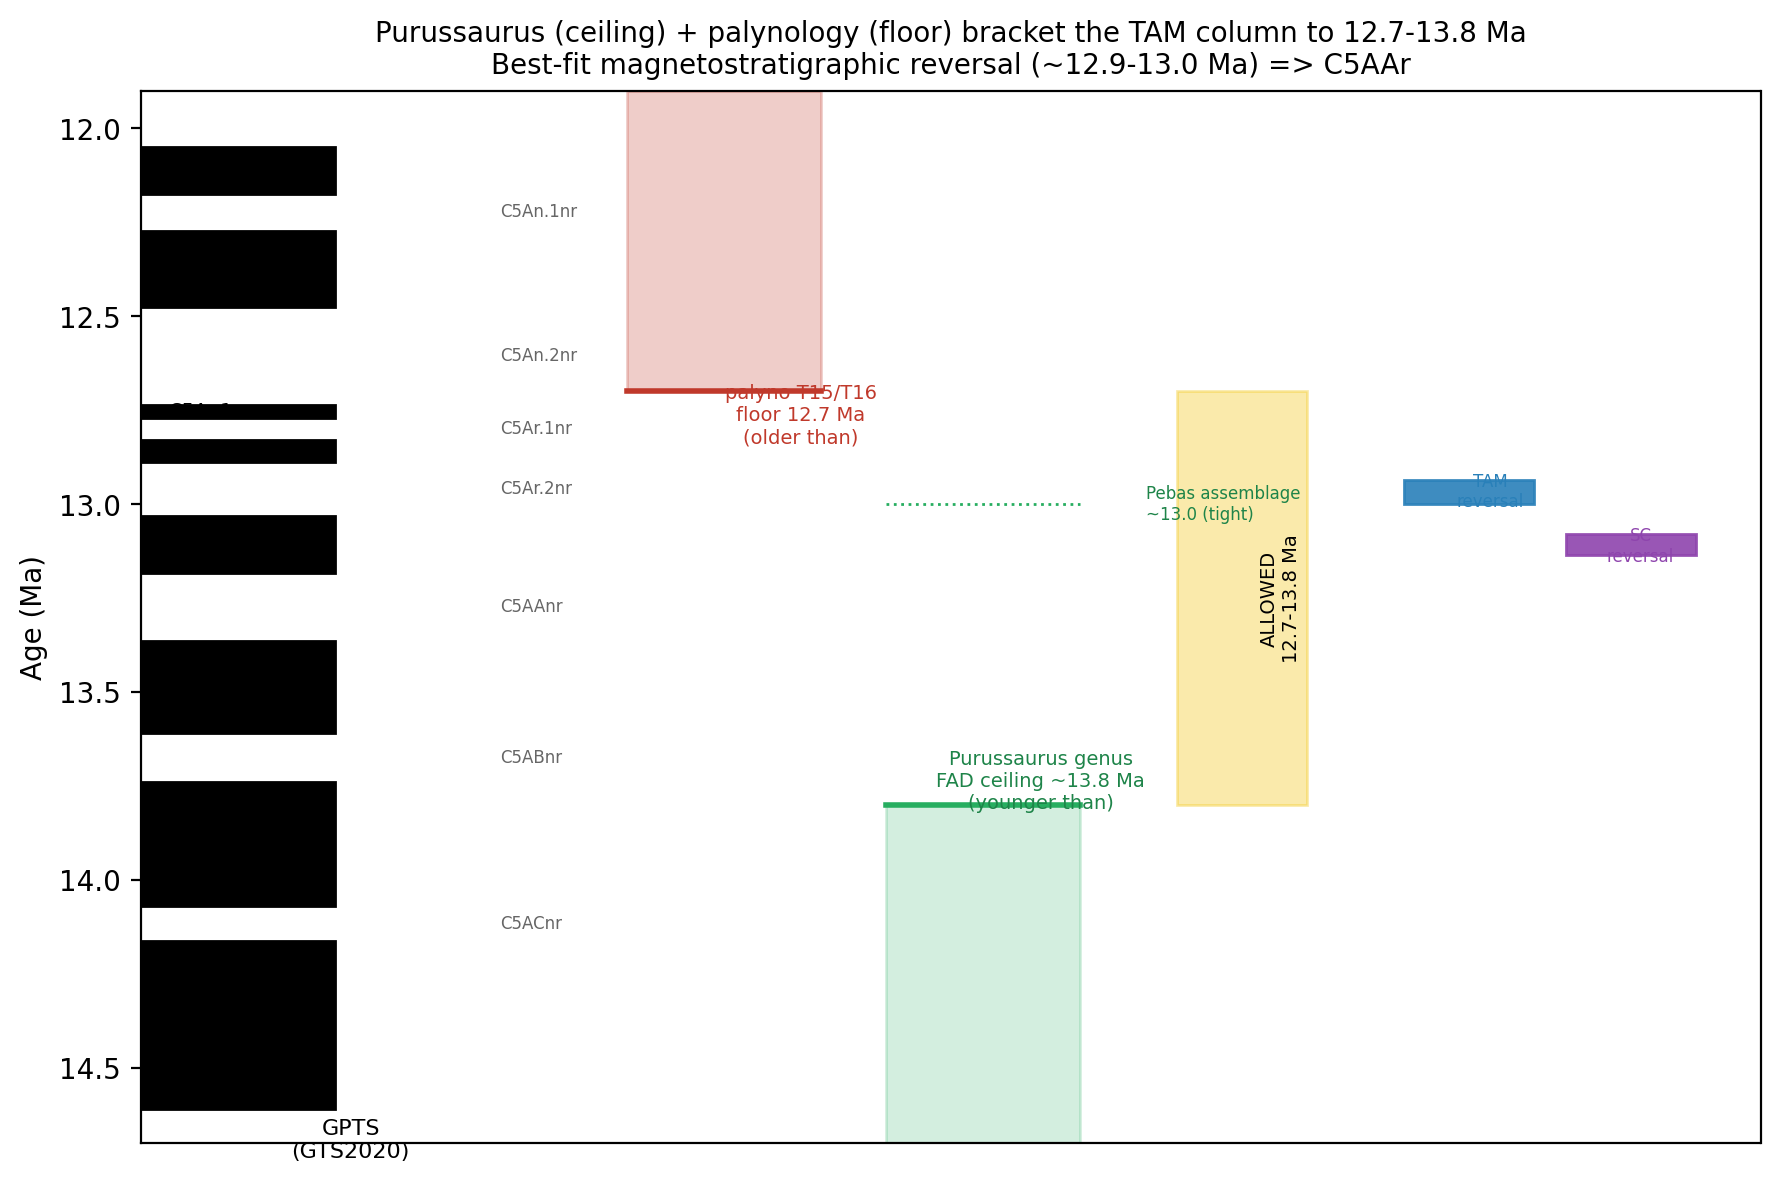
\includegraphics[width=0.72\linewidth]{figs/fig_purussaurus_bracket.png}
\caption{The \textit{Purussaurus} genus ceiling ($<\sim$13.8\,Ma) and the
palynological T-15/T-16 floor ($>$12.7\,Ma) bracket the section to
$\sim$12.7--13.8\,Ma; the tighter Iquitos-Pebas assemblage age ($\sim$13\,Ma)
and La Venta \textit{P.\ neivensis} interval narrow it further. The best-fit
magnetostratigraphic reversal falls at the young edge of this bracket.}
\label{fig:puru}
\end{figure}

\subsection{Regional correlation to La Venta (Honda Group)}\label{sec:laventa}
The strongest \emph{independent} calibration of \textit{Purussaurus neivensis}
comes not from the Pebas (which would be circular) but from La Venta in the
Tatacoa Desert, Colombia, whose Honda Group has recently been re-dated with new
U-Pb zircon geochronology and a Bayesian age--depth model
\citep{MoraRojas2023,Carrillo2023}. In that framework the La Victoria Formation
spans $<$16 to 12.58\,Ma and the Villavieja Formation 12.58 to 10.52\,Ma
(Table~\ref{tab:upb}), and the magnetostratigraphy is reinterpreted as chrons
C5ABn (base) through C5An.1n (top) on the ATNTS2012/GTS2020 scale. Critically,
the fossil-rich ``Monkey Beds'' that yield \textit{P.\ neivensis} are assigned
to chrons \textbf{C5AAr--C5Ar.2n ($\sim$12.83--13.36\,Ma)}. Independently,
\citet{Carrillo2023} note that Laventan-equivalent beds are now recognised at
\emph{Tamshiyacu} itself (near Iquitos), sharing taxa with La Venta.

This lets us tie the Peru record to a regional, radiometrically calibrated
reversal barcode rather than to the abstract GPTS alone (Fig.~\ref{fig:barcode}).
The preferred correlation places the Peru reversal in \textbf{C5AAr}
($\sim$13.2--13.4\,Ma): it satisfies (i) the SC polarity-pattern fit, (ii) the
palynological floor, (iii) the \textit{Purussaurus} ceiling, and (iv) the
U-Pb-dated La Venta \textit{P.\ neivensis} interval, which all overlap at
$\sim$13.2--13.4\,Ma. This converts the earlier tentative $\sim$13\,Ma tie into
one anchored on zircon dates.

\begin{table}[htbp]\centering
\caption{U-Pb zircon ages for the Honda Group (La Venta), from
\citet{MoraRojas2023}. Median and 95\% CI from the Bayesian age model; YSP $=$
youngest statistical population.}
\label{tab:upb}
\begin{tabular}{@{}lrrl@{}}
\toprule
Sample & Strat.\ (m) & Age (Ma, 95\% CI) & Type \\ \midrule
TVV-01 & 932   & 11.5 (10.52--12.09) & detrital MDA \\
SEL-02 & 503   & 12.3 (11.79--12.74) & tuff, YSP 12.8$\pm$0.1 \\
TVV-04 & 474   & 12.3 (11.80--12.77) & tuff, YSP 12.8$\pm$0.1 \\
44011  & 218.8 & 13.1 (12.69--13.47) & tuff, YSP 13.9$\pm$0.3 \\
44017  & 63.5  & 16.0 (15.94--16.00) & tuff, YSP 17.6$\pm$0.4 \\ \bottomrule
\end{tabular}
\end{table}

\begin{figure}[htbp]\centering
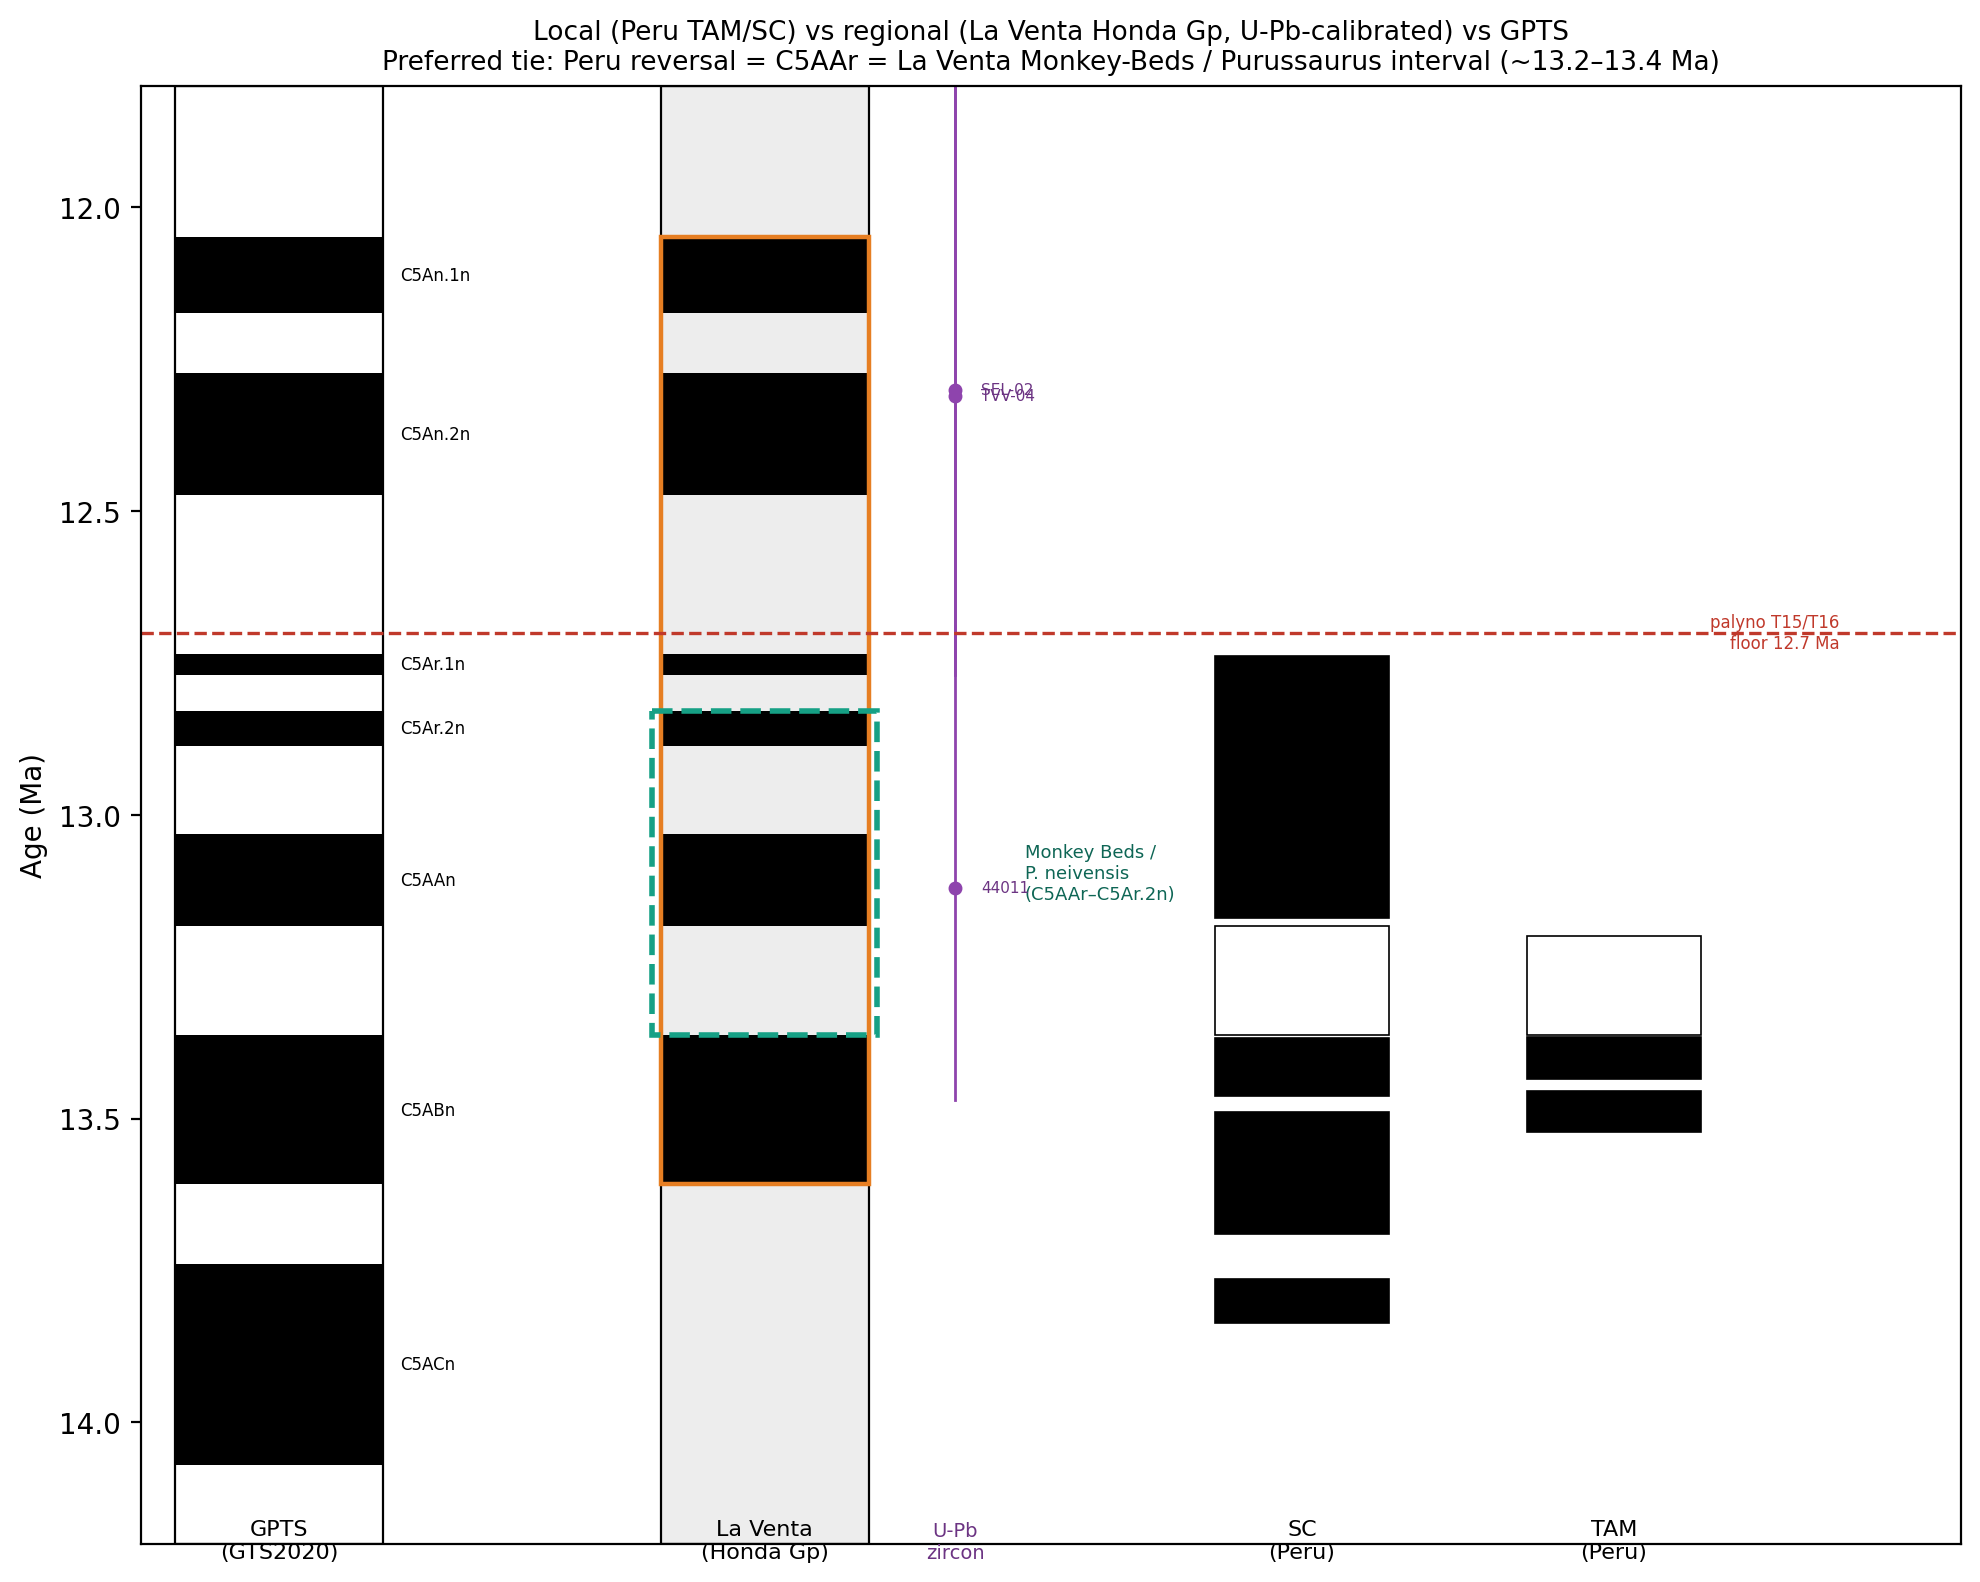
\includegraphics[width=\linewidth]{figs/fig_barcode_comparison.png}
\caption{Local (Peru TAM, SC) vs.\ regional (La Venta Honda Group,
U-Pb-calibrated) vs.\ GPTS (GTS2020) polarity barcodes on a common age axis.
Black $=$ normal. The La Venta column shows the occupied interval (C5ABn--C5An.1n,
orange), the \textit{Purussaurus}-bearing Monkey Beds (C5AAr--C5Ar.2n, green
dashed), and U-Pb sample ages (purple). The Peru reversal aligns with C5AAr and
the La Venta Monkey-Beds interval; the palynological floor (12.7\,Ma, red) bounds
it from below.}
\label{fig:barcode}
\end{figure}

\section{Discussion}

\subsection{Age of the Pebas Formation at Tamshiyacu}
Four independent lines of evidence converge on a middle Miocene age of
$\sim$\SIrange{13.2}{13.4}{\mega\annum} (chron C5AAr) for the studied
succession. (i) The polarity record: each site preserves a single robust
reversal, now expressed antipodally in both inclination and reconstructed
declination, and SC's Normal--Reversed--Normal thickness ratio favours a short
reversed chron between two long normals (C5AAr--C5ABr). (ii) Palynology places
the section in zone T-15 / base T-16, a firm minimum-age (younger-than) bound of
\SI{12.7}{\mega\annum}. (iii) The giant caiman \textit{Purussaurus} supplies the
complementary maximum-age (older-than) bound: the genus does not appear before
$\sim$\SI{13.8}{\mega\annum}. (iv) Most decisively, new U-Pb geochronology from
La Venta \citep{MoraRojas2023} dates \textit{P.\ neivensis} (the same species
reported from the Iquitos Pebas) to chrons C5AAr--C5Ar.2n
($\sim$\SIrange{12.83}{13.36}{\mega\annum}), an anchor independent of the Pebas
itself and therefore free of the circularity that weakens a Pebas-internal
argument. These four constraints overlap only around C5AAr, and the independent
recognition of Laventan-equivalent beds at Tamshiyacu \citep{Carrillo2023}
corroborates the correlation. The middle-Miocene calibration is robust to the
choice of GTS2020/ATNTS2012 vs.\ CK95 (a \SIrange{50}{100}{\kilo\annum} shift),
which is smaller than the current tie uncertainty.

\subsection{Magnetic mineralogy and diagenetic overprinting}
The ChRM is a shallow, dual-polarity, primary detrital remanence, but its
intensity is strongly modulated by diagenesis rather than by the primary
depositional flux of magnetic minerals. NRM intensity tracks susceptibility
($r\approx0.5$--$0.75$) --- both measuring magnetite concentration --- yet is
essentially uncorrelated with XRF total Fe, because in this facies most iron is
locked in \emph{authigenic} phases (pyrite and carbonate; Sec.~\ref{sec:elemstrat})
rather than in detrital magnetite. The most pyritic intervals are also the
lowest in remanence intensity and susceptibility, implying that bacterial
sulphate reduction consumed reactive iron and partly dissolved detrital
(titano)magnetite, driving the low-intensity zones. This is the expected
behaviour of an organic-rich, reducing sediment and it explains why polarity in
those intervals is noise-prone and best read from the surviving high-coercivity
ChRM. It also means XRF Fe cannot substitute for rock-magnetic measurements as a
magnetic-concentration proxy here --- a transferable caution for magnetostratigraphy
in reducing tropical wetland deposits.

\subsection{Redox, pyrite and marine influence in the Pebas mega-wetland}
The elemental stratigraphy records the alternation of environments that defines
the Pebas mega-wetland system. Discrete intervals enriched in S, Fe and Ca
(with Sr) represent \emph{reducing, pyritic, shell-bearing} conditions:
authigenic pyrite (Fe--S) forms where bacterial sulphate reduction operates
below the sediment--water interface, and its abundance is limited chiefly by the
supply of dissolved \emph{sulphate}. In a dominantly freshwater Amazonian system
sulphate is scarce, so the strong, punctuated pyrite enrichments most plausibly
mark intervals of enhanced sulphate availability --- i.e.\ brackish/marine
incursions into the wetland, consistent with the marine-influence signal
independently documented from molluscan \textsuperscript{87}Sr/\textsuperscript{86}Sr
and $\delta$\textsuperscript{18}O \citep[e.g.][]{Wesselingh2006} and with the
Mara\~n\'on-basin incursion interval that spans this time window. The
co-enrichment of Ca and Sr in the same beds --- aragonitic Pebasian mollusc
coquinas --- reinforces this reading: shell beds and pyritic muds are the
sedimentary expression of the same brackish, low-energy, reducing episodes.
Between these episodes, flatter K/Ti and higher Mn indicate more oxygenated,
detritally-diluted freshwater intervals. The section therefore does not record a
single static environment but an oscillation between freshwater-lacustrine and
brackish/marine-influenced states --- the hallmark of the Pebas mega-wetland
during peak inundation.

\subsection{Paleoclimatic and paleogeographic context}
At $\sim$13\,Ma the succession sits immediately after the Middle Miocene
Climatic Transition (MMCT, $\sim$\SIrange{14.2}{13.8}{\mega\annum}), the global
cooling and ice-sheet expansion that ended the Middle Miocene Climatic Optimum.
In western Amazonia this was the time of maximum extent of the Pebas
mega-wetland, when subsiding Andean-foreland accommodation, a low-gradient
landscape and repeated eustatic/relative sea-level pulses combined to admit
brackish waters far into the continental interior. The pyrite--carbonate cycles
we resolve are the local sedimentary fingerprint of that paleogeography: each
marine-influenced interval marks a temporary connection (or restricted-marine
incursion) that raised sulphate and salinity, alternating with freshwater
recovery. Placing these cycles on the magnetostratigraphic age model ties the
Tamshiyacu record into the regional Pan-Amazonian framework (La Venta,
Contamana, the Mara\~n\'on and Solim\~oes basins) at $\sim$13\,Ma and provides a
polarity-calibrated reference against which the timing of individual incursions
can eventually be tested. The subsequent late-Miocene demise of the wetland and
onset of the transcontinental Amazon lies above the studied interval.

\subsection{Limitations and next steps}
The GPTS tie rests on a single well-resolved reversal per site; recovering a
second reversal in one continuous section (e.g.\ confirming the tentative TAM~7
reversal with fuller demagnetisation, or re-measuring the excluded TAM Group~1)
would make the correlation unique rather than best-fit. Species-level
confirmation of the Tamshiyacu \textit{Purussaurus} would convert the vertebrate
constraint from a genus-level ceiling into a tight
($\sim$\SIrange{12.8}{13.4}{\mega\annum}) tie. The azimuth reconstruction would
tighten with a physically fixed reference offset (from confirming the x- vs
y-face convention) and a re-check of the anomalous TAM~6 field azimuth.
Finally, the XRF--environment interpretation is currently qualitative and
depth-registered only approximately; quantitative sulphate/marine-influence
inference would benefit from paired \textsuperscript{87}Sr/\textsuperscript{86}Sr
or S-isotope measurements on the pyritic and shell-bearing intervals identified
here.

\section{Data and code availability}
Processing scripts and derived data (polarity zones, age-model scenarios,
multi-timescale chron tables, fossil-bracket analysis) are archived in the
project repository (\texttt{polarity\_synthesis/}, \texttt{age\_model\_
assessment/}) and in \texttt{Uchannel\_notebook.ipynb}.

\begin{thebibliography}{99}
\small
\bibitem[Carrillo et al.(2023)]{Carrillo2023} Carrillo, J.D., et al., 2023.
The Miocene La Venta Biome (Colombia): a century of research and future
perspectives. \textit{Geodiversitas} 45(26): 741--793.
\bibitem[Cande \& Kent(1992)]{CandeKent1992} Cande, S.C., Kent, D.V., 1992.
A new geomagnetic polarity time scale for the Late Cretaceous and Cenozoic.
\textit{J.\ Geophys.\ Res.} 97, 13917--13951.
\bibitem[Cande \& Kent(1995)]{CandeKent1995} Cande, S.C., Kent, D.V., 1995.
Revised calibration of the geomagnetic polarity timescale for the Late
Cretaceous and Cenozoic. \textit{J.\ Geophys.\ Res.} 100, 6093--6095.
\bibitem[Hilgen et al.(2012)]{Hilgen2012} Hilgen, F.J., Lourens, L.J.,
Van Dam, J.A., et al., 2012. The Neogene Period. In: \textit{The Geologic Time
Scale 2012}, Elsevier, ch.~29.
\bibitem[Hoorn et al.(2010)]{Hoorn2010} Hoorn, C., et al., 2010. Amazonia
through time: Andean uplift, climate change, landscape evolution, and
biodiversity. \textit{Science} 330, 927--931.
\bibitem[Jaramillo et al.(2011)]{Jaramillo2011} Jaramillo, C., Rueda, M.,
Torres, V., 2011. A palynological zonation for the Cenozoic of the Llanos and
Llanos Foothills of Colombia. \textit{Palynology} 35, 46--84.
\bibitem[Jaramillo et al.(2017)]{Jaramillo2017} Jaramillo, C., et al., 2017.
Miocene flooding events of western Amazonia. \textit{Science Advances} 3,
e1601693.
\bibitem[Kirschvink(1980)]{Kirschvink1980} Kirschvink, J.L., 1980. The
least-squares line and plane and the analysis of palaeomagnetic data.
\textit{Geophys.\ J.\ R.\ Astron.\ Soc.} 62, 699--718.
\bibitem[Mora-Rojas et al.(2023)]{MoraRojas2023} Mora-Rojas, L., C\'ardenas, A.,
Jaramillo, C., et al., 2023. Stratigraphy of a middle Miocene neotropical
Lagerst\"atte (La Venta Site, Colombia). \textit{Geodiversitas} 45(6): 197--221.
\bibitem[Pujos \& Salas-Gismondi(2020)]{Pujos2020} Pujos, F.,
Salas-Gismondi, R., 2020. Predation of the giant Miocene caiman
\textit{Purussaurus} on a mylodontid ground sloth. \textit{Biology Letters}
16, 20200239.
\bibitem[Raffi et al.(2020)]{Raffi2020} Raffi, I., et al., 2020. The Neogene
Period. In: \textit{Geologic Time Scale 2020}, Elsevier.
\bibitem[Rebata et al.(2006)]{Rebata2006} Rebata-H., L.A., et al., 2006.
Sedimentology and ichnology of tide-influenced Late Miocene successions in
western Amazonia: the gradational transition between the Pebas and Nauta
formations. \textit{J.\ South Am.\ Earth Sci.} 21, 96--119.
\bibitem[Salas-Gismondi et al.(2015)]{SalasGismondi2015} Salas-Gismondi, R.,
et al., 2015. A Miocene hyperdiverse crocodylian community reveals peculiar
trophic dynamics in proto-Amazonian mega-wetlands. \textit{Proc.\ R.\ Soc.\ B}
282, 20142490.
\bibitem[Wesselingh \& Salo(2006)]{Wesselingh2006} Wesselingh, F.P.,
Salo, J.A., 2006. A Miocene perspective on the evolution of the Amazonian
biota. \textit{Scripta Geologica} 133, 439--458.
\end{thebibliography}

\end{document}
